%-------这是COMAP公司发布的2023年美赛官方LaTeX模板
%-------官方仅提供了summary页面的样式,在此基础上,我们构建一个完整的Template!
%-------下载网站:https://www.comap.com/contests/mcm-icm
%-------E-mail:hnuzyx@outlook.com
%%%%%%%%%%%%%%%%%%%%%%%%%%%%%%%%%%%%%%%%
%% MCM/ICM LaTeX Template %%
%% 2023 MCM/ICM           %%
%%%%%%%%%%%%%%%%%%%%%%%%%%%%%%%%%%%%%%%%
\documentclass[12pt]{article}
\usepackage{xeCJK}
\usepackage{verbatim}


\usepackage[dvipsnames]{xcolor}
%%%%%%%%%%%%%%%%%%%%%%%%%%%%%%%%%%%%%%%%
\usepackage{blindtext}
\usepackage{geometry}
\usepackage{hyperref}
\usepackage{amsmath}
\usepackage{svg} 
\usepackage[T1]{fontenc}
\usepackage{newtxtext}
\usepackage{hyperref}
\usepackage{tabularx}
\usepackage{booktabs}
\usepackage[nottoc]{tocbibind}
\usepackage{pgfplots}
\usepackage{amsmath,amssymb,amsthm}
\usepackage{lipsum}
\usepackage{tikz}
\usepackage{etoolbox}
\usetikzlibrary{trees}
\usepackage{booktabs}
\usepackage{fancyhdr}
\usepackage{listings}
\usepackage{float}
\usepackage{indentfirst}%Latex默认在\chapter和\section等章节标题首段不缩进,加入这个宏包可以解决这个问题
%\usepackage[pdftex]{graphicx}
\usepackage{url}
\usepackage{listings}
% \begin{lstlisting}[language=TeX]
\lstset{
    basicstyle=\sffamily, % 基本代码风格
    keywordstyle=\bfseries, % 关键字风格
    commentstyle=\rmfamily\itshape, % 注释的风格,斜体
    stringstyle=\ttfamily, % 字符串风格
    flexiblecolumns=true, % 别问为什么,加上这个
    numbers=left, % 行号的位置在左边
    showspaces=false, % 是否显示空格,显示了有点乱,所以不显示了
    showstringspaces=false,
    captionpos=t, % 这段代码的名字所呈现的位置,t指的是top上面
    frame=lrtb, % 显示边框
    breaklines=true,
    columns=flexible,
}


\lstdefinestyle{Python}{
    language        =   Python, % 语言选Python
    keywordstyle    =   \color{blue},
    keywordstyle    =   [2] \color{teal},
    stringstyle     =   \color{magenta},
    commentstyle    =   \color{red}\ttfamily,
    breaklines      =   true,   % 自动换行,建议不要写太长的行
    columns         =   fixed,  % 如果不加这一句,字间距就不固定,很丑,必须加
    basewidth       =   0.5em,
}

\newtheorem{theorem}{Theorem}
\newtheorem{corollary}[theorem]{Corollary}
\newtheorem{lemma}[theorem]{Lemma}
\newtheorem{definition}{Definition}
\geometry{left=1in,right=0.75in,top=1in,bottom=1in}
\hypersetup{colorlinks=true, linkcolor=black, urlcolor=black}
%%%%%%%%%%%%%%%%%%%%%%%%%%%%%%%%%%%%%%%%
\lhead{Team \Team}
\rhead{}
\cfoot{}
% Replace ABCDEF in the next line with your chosen problem
% and replace 1111111 with your Team Control Number
\newcommand{\Problem}{D}
\newcommand{\Team}{2321591}
%%%%%%%%%%%%%%%%%%%%%%%%%%%%%%%%
\begin{document}
\graphicspath{{.}}  % Place your graphic files in the same directory as your main document
\DeclareGraphicsExtensions{.pdf, .jpg, .tif, .png}
\thispagestyle{empty}
\vspace*{-16ex}
\centerline{\begin{tabular}{*3{c}}
	\parbox[t]{0.3\linewidth}{\begin{center}\textbf{Problem Chosen}\\ \Large \textcolor{red}{\Problem}\end{center}}
	& \parbox[t]{0.3\linewidth}{\begin{center}\textbf{2023\\ MCM/ICM\\ Summary Sheet}\end{center}}
	& \parbox[t]{0.3\linewidth}{\begin{center}\textbf{Team Control Number}\\ \Large \textcolor{red}{\Team}\end{center}}	\\
	\hline
\end{tabular}}
%%%%%%%%%%% Begin Summary %%%%%%%%%%%
% Enter your summary here replacing the (red) text
% Replace the text from here ...
\begin{center}
%标题
\begin{center}
	\Huge {Multi-Criteria Decision Making for SDGs using K-Means and AHP}
	\vspace{0.4cm}
	
	\normalsize\textbf{Summary}
\end{center}
\vspace{0.2cm}

%下述段落为官方注意事项,写作时注意删除!

\end{center}
% to here



The United Nations has established \textbf{17 Sustainable Development Goals (SDGs)}, which represent humanity's vision for a better future world. These 17 goals may have \textbf{positive or negative impacts} on each other, and therefore, it is crucial to establish a prioritization model for handling these goals. To accomplish this, we require a model that involves both \textbf{network and graph theory} and a model that can determine the most prioritized items.

In Task 1, we constructed a \textbf{network graph} of the 17 SDGs, where we assigned the same color to points representing goals belonging to the same category and used lines to indicate their relationships. To avoid the intersection of points and lines, we let the 17 targets form a circle, so that our diagram will look clearer.

In Task 2, we used the traditional \textbf{Analytic Hierarchy Process (AHP)} method to establish a model for selecting the optimal goal from the 17 SDGs. First, we provided 5 criteria for evaluating the goals as the decision layer, and then the 17 SDGs as the alternative layer. By comparing the judgment matrices through the \textbf{AHP algorithm}, we obtained the evaluation weights of the 5 criteria and the priority levels (represented by numerical values) of each goal. The goal with the highest priority value was considered the most prioritized item.

In Task 3, we aimed to determine the new most prioritized item after a particular goal had been accomplished. Considering that the traditional AHP method would result in complicated operations and substantial human input, and that removing a goal would require changing the parameters of the original matrix, we used the \textbf{K-Means clustering algorithm} to classify the 17 goals. After classifying the goals, we placed goals from the same class in the same\textbf{ AHP alternative layer}, and each class's local most prioritized item was determined. Finally, we included these local most prioritized items in the\textbf{ AHP model }to determine the overall most prioritized item.

In Task 4, due to unexpected events, we realized that the original decision layer might no longer be appropriate, so we replaced it with the United Nations' official \textbf{5P classification} for the 17 SDGs to adapt to the new situation. The other procedures were similar to those in Task 3. Here we discuss what happens to the 5Ps, which are indicators at the decision-making level, when economic, technological, political, and environmental factors change; we also plot pie charts comparing these changes to the original state.

In Task 5, we discussed in detail what kind of problems other companies and organizations can solve using our model and how to solve them using our model. We also considered other situations that might arise in practical problems, and therefore, we provided optimization suggestions for these situations.

Finally, we conducted sensitivity analysis, analyzed the strengths and weaknesses of the model, and provided prospects for the model's future development.


\begin{comment}

联合国制定了17项可持续发展目标,它们代表着人类对于未来世界的美好愿景。这17项目标相互之间可能有着影响,积极的或者是消极的。处理这些目标需要有一个先后顺序,那么确定最为优先的事项就显得尤为重要。因此我们需要一个有关图与网络的模型和一个能够确定最优先事项的模型。

在任务一中,我们构建了一个关于17个可持续发展目标的网络图,在这个图中我们根据17个目标的分类,给相同的目标所代表的点涂上一样的颜色,并且使用连线来表示他们相互之间的关系。为了避免出现点与线的交错,我们让这17个目标围成一圈,这样子我们的图看起来就会比较清楚。

在任务二中,我们使用传统的AHP方法来构建从17个目标中取得最优目标的模型。首先我们给定了5个评价目标的标准作为AHP的决策层,然后17个目标作为方案层。这样子通过AHP的比较判别矩阵的算法来求解出5个评价标准的评价权重以及每个目标的优先程度(通过数值来表示),这样子优先程度数值最高的就成为了优先考虑事项。

在任务三中,我们需要考虑如果某个目标被完成之后,新的最优先事项是什么。考虑到传统的AHP方法会带来比较繁琐的运算和庞大的人为赋值,同时一个目标被移除会导致原矩阵的参数需要变动,因此我们使用K-Means聚类算法来进行17个目标的分类。分好类之后我们将同类的目标放进AHP的方案层里面,不同的目标不同时放进,这样子每一类的局部最优先事项就可求出。最后再将这些局部最优先事项放进AHP中,得到最优的事项。

在任务四中,由于出现了一些突发事件,因此我们考虑到原先的决策层可能不再适用,因此我们选择将原来的决策层更换为联合国官方为17个目标做的分类5Ps,这样子就可以适应于新的情境。而其他的操作和任务三差不多。在这里我们讨论了当经济、科技、政治、环境因素发生变化的时候,作为决策层指标的5Ps会发生什么变化;同时我们将这些变化与原先状态下进行比对,绘制了饼图。

在任务五中,我们详细讨论了其他的公司和组织可以通过我们的模型解决什么样的问题,如何通过我们的模型解决问题。同时我们考虑到实际的问题中可能会出现的其他的情况,因此后面对于任务5的表述中也会提到对于这一种情况我们提出了什么样的优化建议。

最后,我们进行了灵敏度分析,同时分析了模型的优缺点,最后进行了对于该模型的未来展望。

\end{comment}



%关键词
\vspace{0.4cm}
\noindent \textbf{Keywords:}\quad 17 SDGs \quad Graph and Network \quad Analytic Hierarchy Process(AHP) \quad K-Means cluster algorithm \quad 5P classification
%%%%%%%%%%% End Summary %%%%%%%%%%%

%%%%%%%%%%%%%%%%%%%%%%%%%%%%%%
\clearpage
\pagestyle{fancy}
% Uncomment the next line to generate a Table of Contents
%\tableofcontents 
\newpage
\setcounter{page}{1}
\rhead{Page \thepage~of~25}
%%%%%%%%%%%%%%%%%%%%%%%%%%%%%%
%目录
\tableofcontents
\newpage

%正文部分
\section{Introduction}
\subsection{Problem Background}

\begin{comment}
伴随着人类的发展,我们的生活水平和生活质量不断提高,但是在我们这个广大的世界之中,我们依然面临了诸多问题。联合国组织总结出了17个可持续发展的核心目标,这些问题有着不同的侧重点,但是他们都是我们最为重要的议题


联合国发展到今天,我们面临了许多问题这些问题有大有小,我们需要解决。
但同时,有一些问题伴随了人类历史这么多年,需要我们着重进行考虑。这些问题概括了人类历史发展的诸多问题挑战。他们有17个,我们称之为17个可持续发展问题。、
这些可持续发展问题有:
目标1:无贫困\\
目标2:零饥饿\\
目标3:良好的健康和福祉\\
目标4:优质教育\\
目标5:性别平等\\
目标6:清洁水和卫生\\
目标7:负担得起的清洁能源\\
目标8:体面的工作和经济增长\\
目标9:工业、创新和基础设施\\
目标10:减少不平等\\
目标11:可持续的城市和社区\\
目标12:负责任的消费和生产\\
目标13:气候行动\\
目标14:水下生命\\
目标15: 陆地生物\\
目标16:和平与正义强大的机构\\
目标17:实现目标的伙伴关系\\

如此之多的目标问题,我们需要进行分析,以便得到最终的解决方案,来让人类社会变得更加美好。
\end{comment}


The 17 Sustainable Development Goals (SDGs) are not standalone objectives, but rather a network of interdependent goals that interact with each other in various ways. The success of achieving one goal often depends on the success of achieving other goals. For instance, ensuring access to clean water and sanitation (SDG 6) is critical to reducing poverty (SDG 1) and improving health and well-being (SDG 3). Similarly, promoting affordable and clean energy (SDG 7) is essential to combatting climate change (SDG 13) and promoting sustainable cities and communities (SDG 11).

Conversely, the failure to achieve one goal can also hinder progress towards other goals. For example, if education (SDG 4) is not accessible to all, then achieving gender equality (SDG 5) and reducing poverty (SDG 1) become more difficult. Moreover, the failure to address climate change (SDG 13) may exacerbate hunger (SDG 2) and limit the availability of clean water and sanitation (SDG 6).

Therefore, it is essential to recognize the interconnectedness of the SDGs and address them holistically, rather than separately. To achieve sustainable development, we must prioritize integrated approaches that consider the impacts of achieving one goal on other goals. This requires collaboration and partnerships among governments, international organizations, civil society, and the private sector to develop strategies and implement solutions that address the interrelated challenges faced by the world. By working together and taking a systemic approach, we can achieve the SDGs and create a better world for all.



\begin{figure}[h]%插入图片并且加上图片的标题,这是一个模板
    \centering
    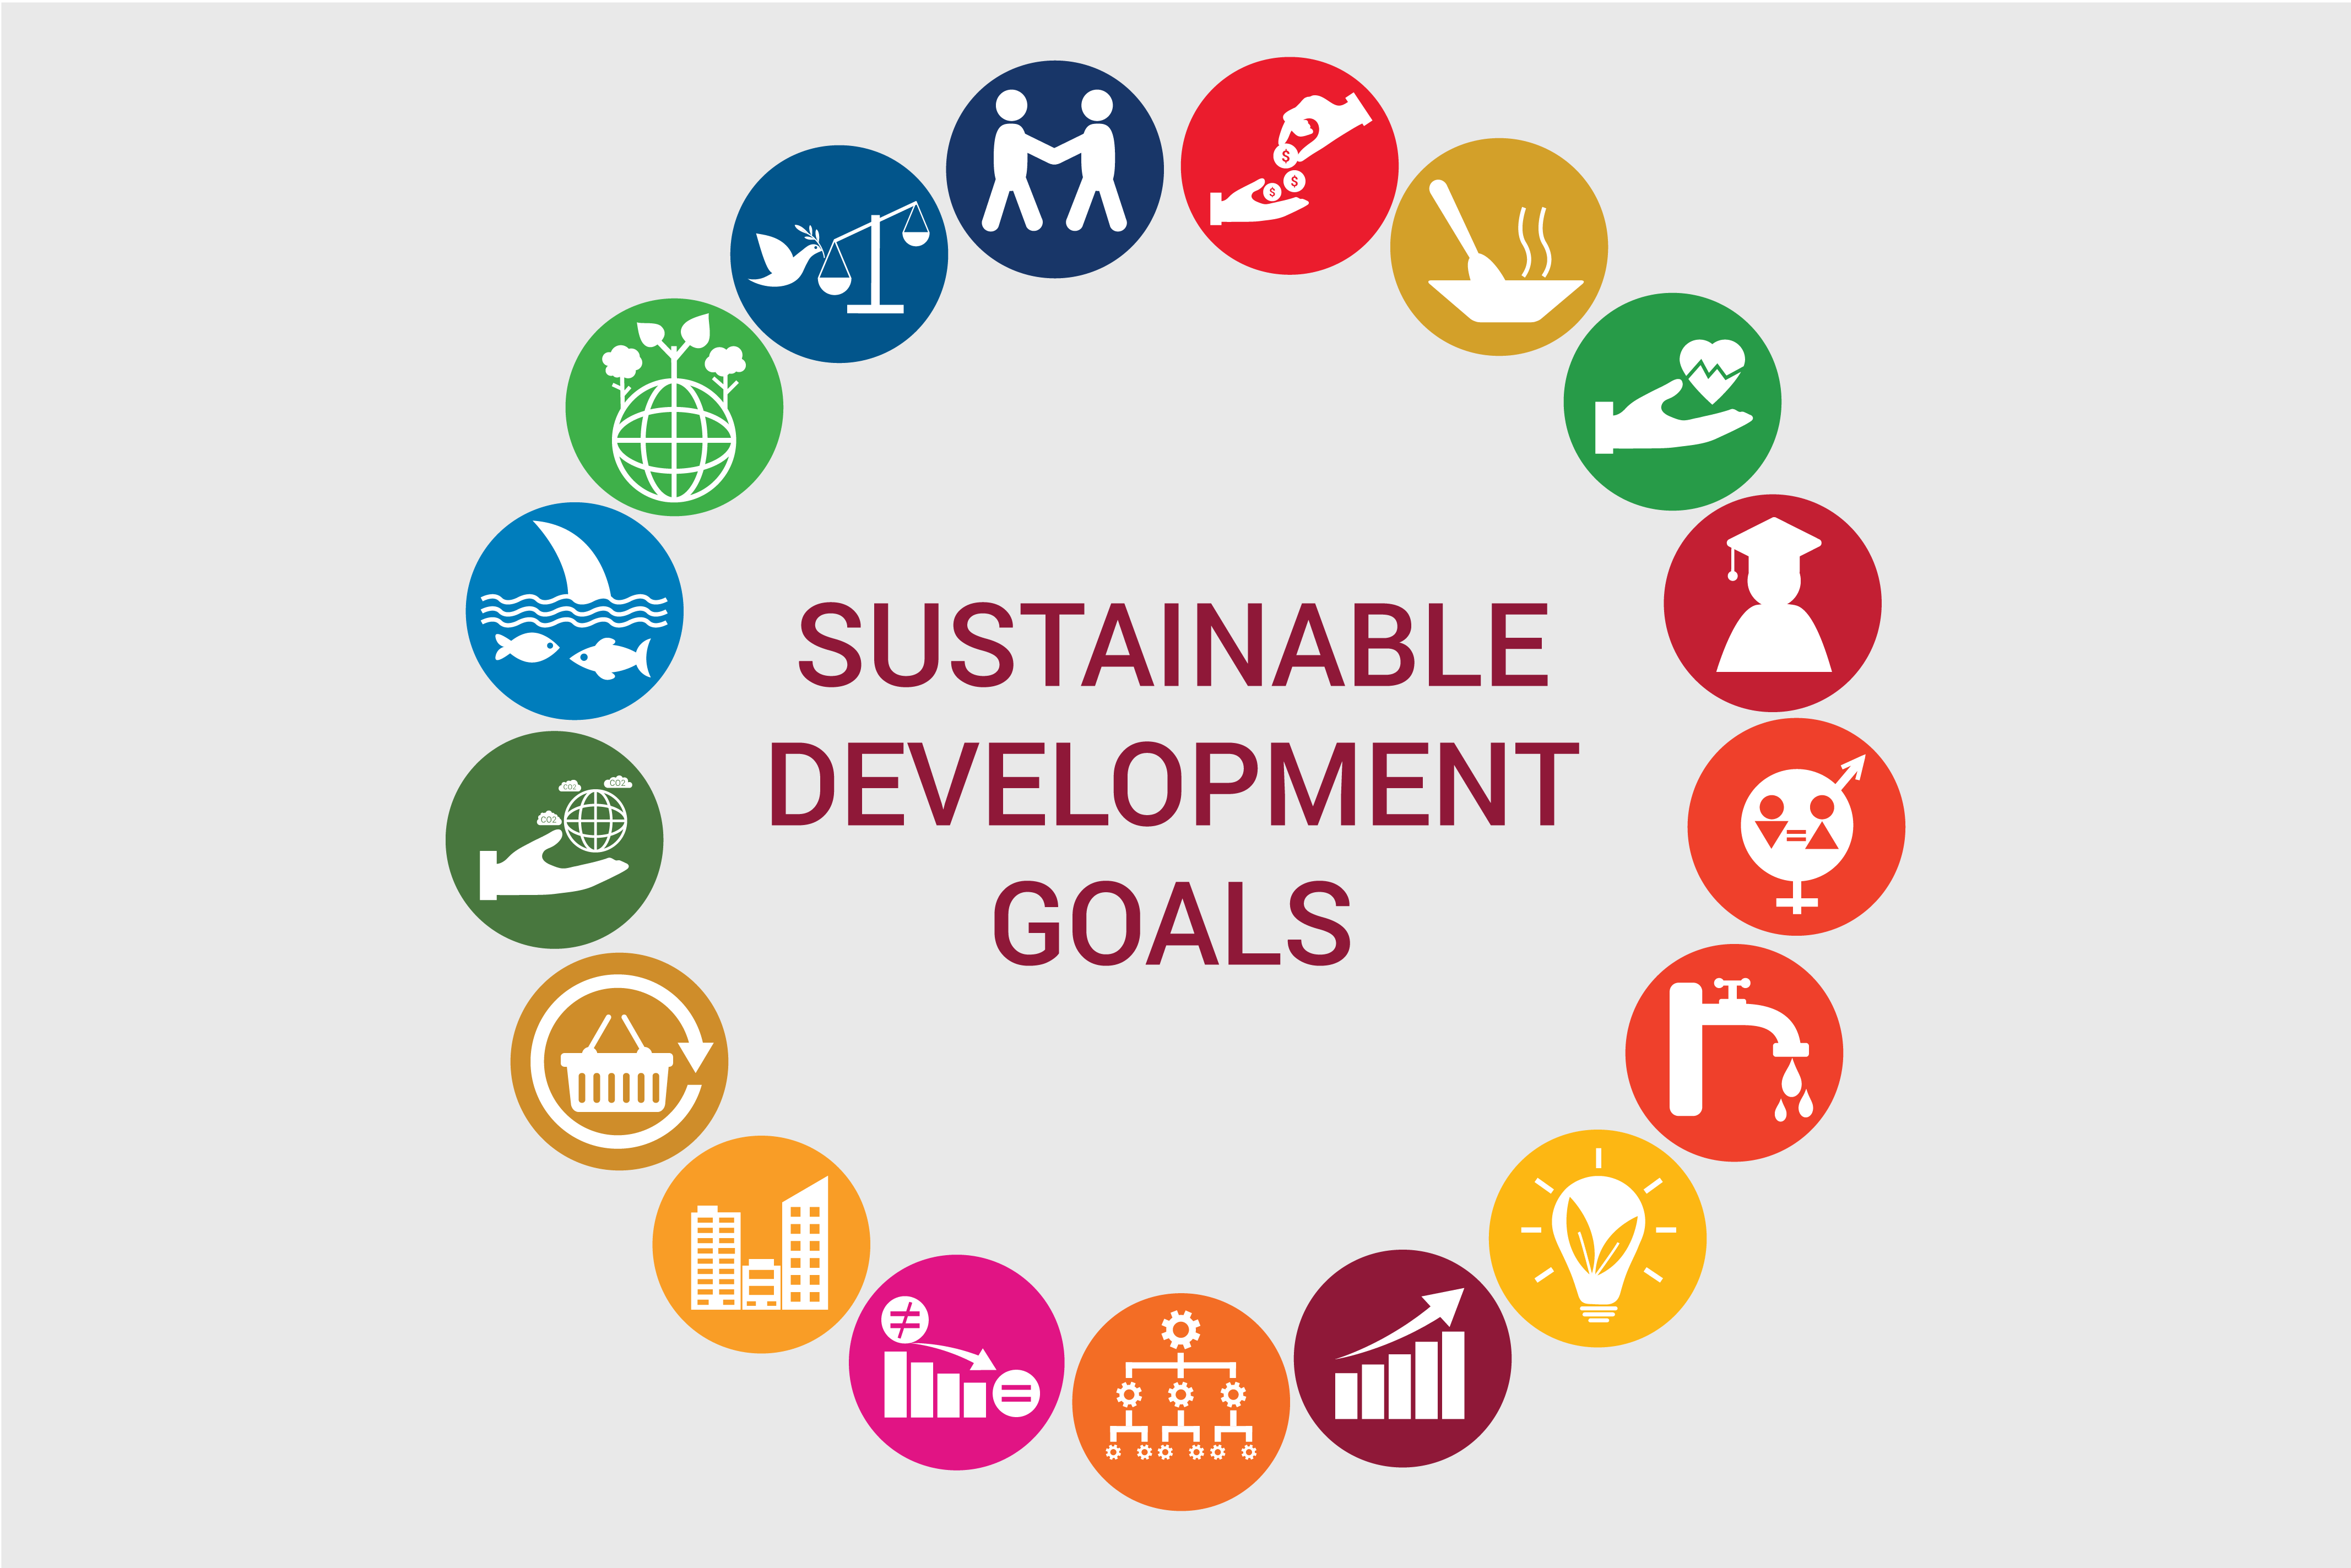
\includegraphics[scale=0.06]{{figure/SDGs.png}}%插入图片的指令
    \caption{The 17 SDGs of UN}%标题
    \label{Label}
\end{figure}



\subsection{Restatement of the Problem}



Considering the background information and restricted conditions identified in the problem statement, we need to establish a model that is universal in its applicability to different athletes and complete the following tasks using the model:    
\begin{itemize}
    \item \textbf{In Task 1} We need to create a \textbf{network} of relationships among the 17 SDGs. Since each of these 17 goal relationships has its own uniqueness, we treat each of the 17 goals as 17 nodes of the network and construct the undirected network. In a certain two nodes, i.e., between certain two goals, there is a unique relationship function. We indicate that they have certain connections by connecting lines in the relational network. The details are described in Task 1.
    
    
    \item In \textbf{Task 2}, We need to use the individual SDGs as well as the network structure to set priorities, and we need to prioritize each event. This task requires a generalization of the 17 SDGs, as well as a decision model that can effectively calculate priorities and make stage-by-stage projections of future development trends.
    

    \item In \textbf{Task 3}, We need to test the scalability of the model. We need to consider how the structure of our network will change when one of the SDGs is achieved. We need to compare the structural changes in the network model before and after the hypothesis, as well as think about related issues that may occur in the future, and suggest possible sustainability topics that may arise in the future.
    
    \item \textbf{In Task 4}, We need to think about the evolution of models under special events. When global progress or major disasters occur, we need to explore the changes in the model and how these changes affect the results of our model calculations, i.e., the priorities of the Sustainable Development Goals. We also need to think about how these changes will affect the future of the UN.
    
    \item \textbf{In Task 5}, We need to extend the model and explore how it can be extended from the 17 UN Sustainable Development Goals to other companies or organizations for goal prioritization.


\end{itemize}
\subsection{Overview of Our Work}

\begin{comment}
我们对任务的背景进行了分析,并建立了模型进行生长预测。我们首先建立了基于单个生菜的生长干重模型。我们对光照和温度两大主要因素进行估计分析,建立了单个生菜的生长模型。我们基于这个单体生长模型,延伸出了有限空间内的年生长鲜重模型。我们思考了种植密度和收获策略,得到了可以在有限集装箱中收获最多生菜鲜重的模型。随后我们加入了集装箱生产的耗能分析,建立了植物工厂完整的生菜生产模型。在这个模型中,我们考虑了照明强度,温度,照明时间等等,并按照生产热量作为分析依据,模拟出了植物工厂的能源消耗。并以机械通风为样本,分析了机械通风的运行策略,并且评估其节能潜力。



\end{comment}

\begin{figure}[h]%插入图片并且加上图片的标题,这是一个模板
    \centering
    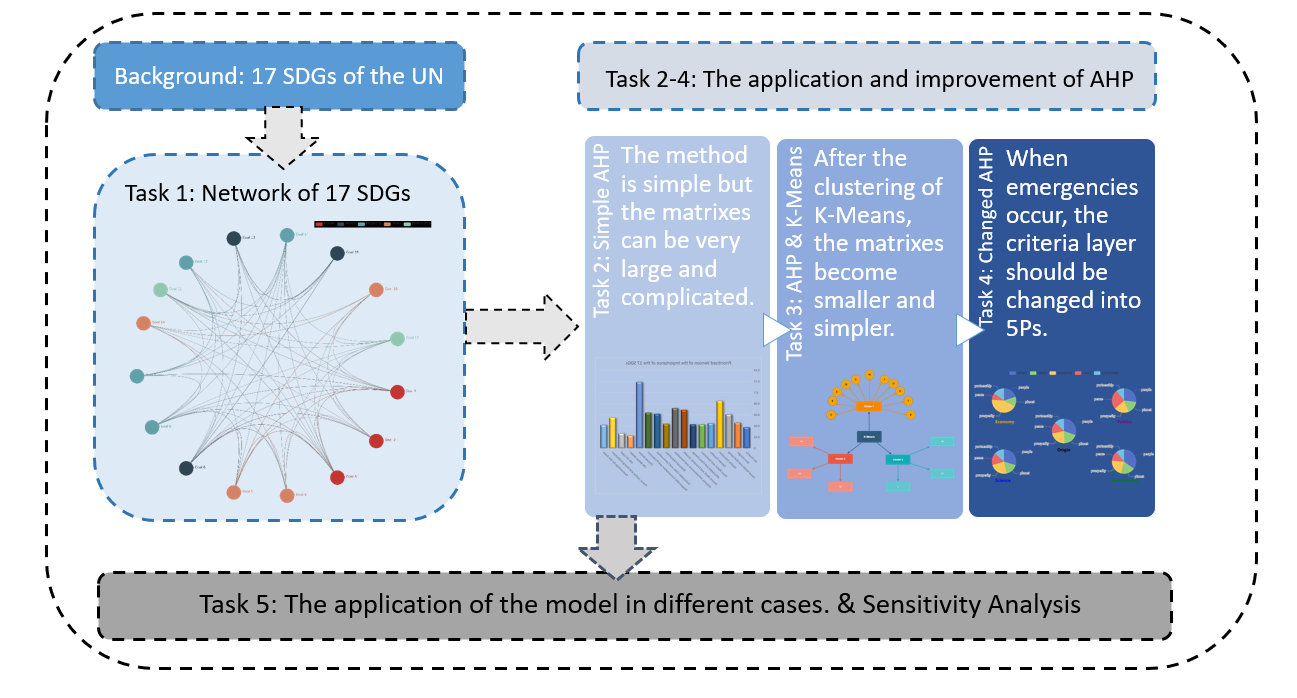
\includegraphics[scale=0.59]{{figure/LiuCheng.png}}%插入图片的指令
    \caption{Our Work Structure}%标题
    \label{Label}
\end{figure}


\section{Assumptions and Notations}

\subsection{Assumptions}

\begin{itemize}
    \item \textbf{Task1: }
    
    Provide a growth model describing the fresh weight of individual lettuce as a function of light intensity and temperature.
  
    \textbf{Justifications:}
    
    \begin{comment}
        任务要求我们分析单个生菜的生长鲜重。因此模型的最终因变量为生菜的鲜重。同时该任务要求我们分析两个因素,分别为光照和温度。我们根据常识猜测,光照与温度两个因素相关性较小,而根据相关文献,我们发现两者处于弱相关,这与我们的猜想符合的很好。因此我们分别假设光照和温度的影响函数相互独立,并在计算鲜重时将其相乘从而进行相关性计算。根据相关数据,我们进行了拟合和归一化计算,得到了最终模型。和测试数据符合的很好。
    \end{comment}

    The task required us to analyze the fresh weight of individual lettuce growth. Therefore the final dependent variable of the model is the fresh weight of lettuce. The task also required us to analyze two factors, namely light and temperature. We guessed based on common sense that the two factors, light and temperature, are less correlated, and based on the relevant literature, we found that they are in a weak correlation, which is in good agreement with our guess. Therefore, we assumed that the effect functions of light and temperature were independent of each other, respectively, and multiplied them in the calculation of fresh weight thus performing the correlation calculation. Based on the correlation data, we performed the fitting and normalization calculations to obtain the final model. It fits well with the test data.
    
    \item \textbf{Task2: }
    
    Considering the planting density and harvesting strategy, please give a model to depict the annual fresh weight of harvested lettuce that can be yielded in the space of a 20-foot container. Assume that the climatic parameters are consistent with the external environment, and the light can be uniformly distributed in the inner area. Lettuce can be harvested when its weight reaches between 250 g and 500 g.
  
    \textbf{Justifications:}
    
    \begin{comment}
        任务要求我们分析一定尺寸的集装箱内生菜生长的年鲜重。我们在任务一中已经得到了单个生菜生长的基本模型,在这里对任务1中的模型进行再次利用即可。我们对单个个体的吸收资源和土地的总资源进行假设,因此可以得出适宜的种植密度,该密度也和工厂的面积相关,该面积为常熟。当密度较小时,我们认为每个个体达到自身吸收的最大值,而当密度较大时,个体吸收资源相同,均分总资源。由此我们可以得到吸收资源与种植总密度的关系,结合任务一中的模型,就可以得到最终的年鲜重模型。
    \end{comment}

    The task requires us to analyze the annual fresh weight of lettuce grown in a container of a certain size. We have already obtained the basic model for the growth of individual lettuce in Task 1, and it is sufficient to reuse the model from Task 1 here. We make assumptions about the absorption resources of individual individuals and the total resources of the land, so that we can derive a suitable planting density, which is also related to the area of the plant, which is constant. When the density is small, we consider that each individual reaches the maximum of its own absorption, while when the density is large, the individual absorption resources are the same and the total resources are equally divided. From this we can obtain the relationship between the absorbed resources and the total planting density, and combined with the model in Task 1, we can obtain the final annual fresh weight model.
    
    \item \textbf{Task3: }
    
   Considering the energy consumption in a 20-foot container plant factory. Please develop: 
    \begin{itemize}
       \item[$\diamond$]A model for calculating annual air conditioning energy consumption of a container factories plant as a function of temperature, insulation material (Appendix B), orientation, planting density, and duration of photo-/dark period (for lettuce, 16h for photo-period and 8h for a dark period); and
       \item[$\diamond$]A model for calculating the lighting energy consumption of a container factories plant as a function of the intensity of the artificial lighting and planting density.
    \end{itemize}


  
    \textbf{Justifications:}
    
    \begin{comment}
        任务要求我们分析工厂的能耗。工厂的能耗可以综合考虑为热量损耗,包括热量产生和热量浪费。热量产生主要有照明耗热和空调耗热,而后者并没有在此任务中要求,而是在任务四和五中进行计算分析。热量浪费主要是材料导热。分析热量产生的过程,我们可以假定一定的照明时间和工厂所需要的摄氏温度。同时,我们也要考虑外界的温度和材料的导热能力。材料的导热能力主要是材料密度,热导率和比热容三个因素。需要注意的是,我们的工厂是一个长方体,因此我们也要考虑工厂与南北纬度的夹角。至此,我们已经总结了工厂的主要能耗因素。工厂照明时,我们对照明灯光强进行假设,即可完成能量损耗的分析模型。我们再次进行了一个基本假设,即工厂先因其他条件到达一个温度,而后在不考虑其他影响下空调单独工作使温度到达预设温度,所以空调消耗可视作以一天为一个单位。
    \end{comment}

    The task requires us to analyze the energy consumption of the plant. The energy consumption of a factory can be considered as a combination of heat loss, including heat generation and heat waste. Heat generation is mainly lighting heat consumption and air conditioning heat consumption, while the latter is not required in this task, but is calculated and analyzed in tasks 4 and 5. Heat wastage is mainly material heat conduction. To analyze the process of heat generation, we can assume a certain lighting time and the required Celsius temperature of the plant. Also, we have to consider the outside temperature and the thermal conductivity of the material. The thermal conductivity of the material is mainly three factors: material density, thermal conductivity and specific heat capacity. It is important to note that our plant is a rectangle, so we also have to consider the angle of the plant to the north and south latitudes. At this point, we have summarized the main energy consumption factors of the factory.The analytical model of energy loss is completed by making assumptions about the light intensity of the lighting when lighting the plant. Again, we make a basic assumption that the plant reaches a temperature first due to other conditions, and then the air conditioner works alone to reach a preset temperature without considering other effects, so the air conditioner consumption can be considered as a unit of one day.
    
    
    \item \textbf{Task4 \& 5: }
    \begin{itemize}
         \item[$\diamond$]Based on the models obtained from the above questions, please build a model that can predict the energy consumption per fresh weight of lettuce. Describe how the energy consumption per yield is affected by the design factors, such as planting density, lighting intensity, temperature, insulation materials, orientation, and duration of a photo-/dark period. Please offer an optimal design and operational strategy to balance yield and energy consumption.
    
        \item[$\diamond$]One proposed solution to reduce the energy consumption of air conditioners is to use ventilation when the external climate conditions are suitable. Because natural ventilation is unstable, mechanical ventilation driven by a fan can be applied. The energy consumption of mechanical ventilation is related to the ventilation rate provided by the fan and is usually much lower than that of an air conditioner. The maximum air change rate of mechanical ventilation can be assumed as two times per hour. Please develop a model to determine the operation strategy for mechanical ventilation and evaluate its energy-saving potential.
    \end{itemize}
    
    \textbf{Justifications:}
    
    \begin{comment}]
    任务四要求我们考虑工厂的照明损耗,并根据能耗的情况选择相应的材料。而根据我们前面的基本模型,可以较为轻松的应用在这两个人物之中。我们假定照明的时间,并在照明函数中进行自变量的扩展,从而轻松得到全新的险种计算函数。为了平衡产量和能源消耗,我们假定二者的权重一样,从而可以根据任务三的模型计算出相应的变量,得到最终的结果演示。任务五要求我们考虑工厂的能量情况,并考虑机械通风的利用度。我们考虑了机械通风的协调性和资源的情况,可以轻松地分析最终的节能潜力。
    \end{comment}
    
    Task 4 requires us to consider the lighting losses of the factory and to choose the appropriate materials according to the energy consumption. And according to our previous basic model, it can be applied to both characters with relative ease. We assume the timing of lighting and extend the independent variables in the lighting function to easily obtain a completely new risk calculation function. To balance production and energy consumption, we assume the same weights for both, so that we can calculate the corresponding variables according to the model of task three and get a demonstration of the final results. Task V requires us to consider the energy profile of the plant and to consider the degree of utilization of mechanical ventilation. We consider the coordination of mechanical ventilation and the resources, and can easily analyze the final energy saving potential


\end{itemize}



\subsection{Notations}

\begin{table}[h]
	\begin{center}
		\begin{tabular}{ccc}
			\toprule[1.5pt]
			Symbol&Definition&Unit\\
			\midrule[1pt]
			\(m\)&Individual lettuce final fresh weight&g\\ 
			\(T\)&Temperature of a single lettuce &℃\\
			\(l\)&light intensity&cd\\
			\(S\)&Total land resources&J\\
			\(s_0\)&Land resources absorbed by a single individual&J\\
			\(\rho\)&planting density&tree/$m^2$\\
			\(c\)&Area of the factory&$m^2$\\
			\(T_0\)&Required temperature of lettuce&℃\\
			\(\rho(n)\)&Material density&kg\cdot{$m^{-3}$}\\
			\(\lambda(n)\)&Thermal conductivity&{W\cdot$m^{-2}$\cdot$K^-1$}\\
			\(c(n)\)&Specific heat capacity&{kJ\cdot$kg^{-1}$\cdot$K^{-1}$}\\
			\(m(n)\)&Total mass of container&kg\\
			\(V\)&The Volume of container shell&$m^3$\\
			
			\(p_0\)&Power required for the lamp to provide 1cd light intensity&W\cdot$h^{-1}$\\
			\(E\)&Total required energy&J\\
            \(W_1\)&The energy exchanged by container and outside air&J\\
            \(W_2\)&The lamp lighting power&J\\
            \(q_0\)&The heat required to increase 1 ℃ per cubic meter of air&J\\
            \(T_1\)&The outside temperature&℃\\
            \(Q_{out}\)&The total energy that the container absorbed&J\\
            \(Q_{sun}\)&The energy that the container absorbed from the sun&J\\
            \(Q_{light}\)&The energy that the container absorbed from the lights&J\\

            
			\bottomrule[1.5pt]
		\end{tabular}
	\end{center}
\end{table}

\begin{table}[h]
    \begin{center}
        \begin{tabular}{ccc}
        \toprule[1.5pt]
			Symbol&Definition&Unit\\
			\midrule[1pt]
            \(S_e\)&The effective area of solar irradiation&$m^2$\\
            \(q_1\)&The heat per unit area of the sum hitting the earth&J\\
            \(S_0\)&The factory area&$m^2$\\
            \(y\)&Wall thickness of the container&m\\
            \(T_2\)&The temperature of the outer surface of the factory&℃\\
            \(P_{static}\)&Fan resting power&W\\
            \(P_{dynamic}\)&Fan movement power&W\\
            \bottomrule[1.5pt]
    \end{tabular}
    \end{center}
\end{table}
% 这一部分是表格,我们在这里罗列我们写的参数,需要列一下
% 如果时间充裕,列一下数据,另外起一个subsection


\section{Task1: Network Model based on Network Flows}% 基于网络流
%任务一需要我们完成一个17节点的网络。根据文章给出的信息,17个节点是联合国官方提出的17个可持续发展目标。他们已经在文章的1.1部分叙述过,因此我们在此按照Goal1,2 ... 17 的名字来代替他们。
Task one requires us to complete a 17-node network. According to the information given in the article, the 17 nodes are the 17 sustainable development goals officially proposed by the United Nations. They have already been described in section 1.1 of the article, so we follow Goal 1,2 here... 17 names to replace them.

%根据联合国官方公布的相关论文信息,我们可以将17个可持续发展目标分为5个大类,也即5个P。它们分别是:People,Prosperity,Peace,Planet 和 Partnership。这5个P一起囊括了这17个可持续发展目标。当然,这并不意味着每一个目标相互独立,相反,每一个目标和5Ps都有着或多或少的关系,只是根据其主要囊括内容进行分类。
According to the official United Nations paper, we can classify the 17 SDGs into 5 broad categories, namely the 5 Ps: \textbf{People, Prosperity, Peace, Planet and Partnership}, which together encompass the 17 SDGs. Of course, this does not mean that each goal is independent of the other, rather, each goal is more or less related to the 5 Ps, but is classified according to its main content.

The 17 Sustainable Development Goals (\textbf{SDGs}) outlined in the 2030 Agenda for Sustainable Development can be classified into the following \textbf{5 Ps} based on the official report on un.org:


% \begin{table}[htbp]
%   \centering
%   \caption{SDGs by Categories}
%     \begin{tabularx}{\textwidth}{XX}
%     \toprule
%     \textbf{People} & \textbf{Planet} \\
%     \midrule
%     SDG 1: No Poverty & SDG 7: Affordable and Clean Energy \\
%     SDG 2: Zero Hunger & SDG 9: Industry, Innovation and Infrastructure \\
%     SDG 3: Good Health and Well-being & SDG 11: Sustainable Cities and Communities \\
%     SDG 4: Quality Education & SDG 12: Responsible Consumption and Production \\
%     SDG 5: Gender Equality & SDG 13: Climate Action \\
%     SDG 6: Clean Water and Sanitation & SDG 14: Life Below Water \\
%     SDG 10: Reduced Inequalities & SDG 15: Life On Land \\
%     SDG 16: Peace, Justice and Strong Institutions & \\
%     \bottomrule
%     \end{tabularx}%
%   \label{tab:addlabel}%
% \end{table}%

% \begin{table}[htbp]
%   \centering
%   \caption{SDGs by Categories}
%     \begin{tabularx}{\textwidth}{XXX}
%     \toprule
%     \textbf{Prosperity} & \textbf{Peace} & \textbf{Partnership} \\
%     \midrule
%     SDG 8: Decent Work and Economic Growth & SDG 16: Peace, Justice and Strong Institutions & SDG 17: Partnerships for the Goals \\
%     \bottomrule
%     \end{tabularx}%
%   \label{tab:addlabel}%
% \end{table}%
\begin{figure}[h]%插入图片并且加上图片的标题,这是一个模板
    \centering
    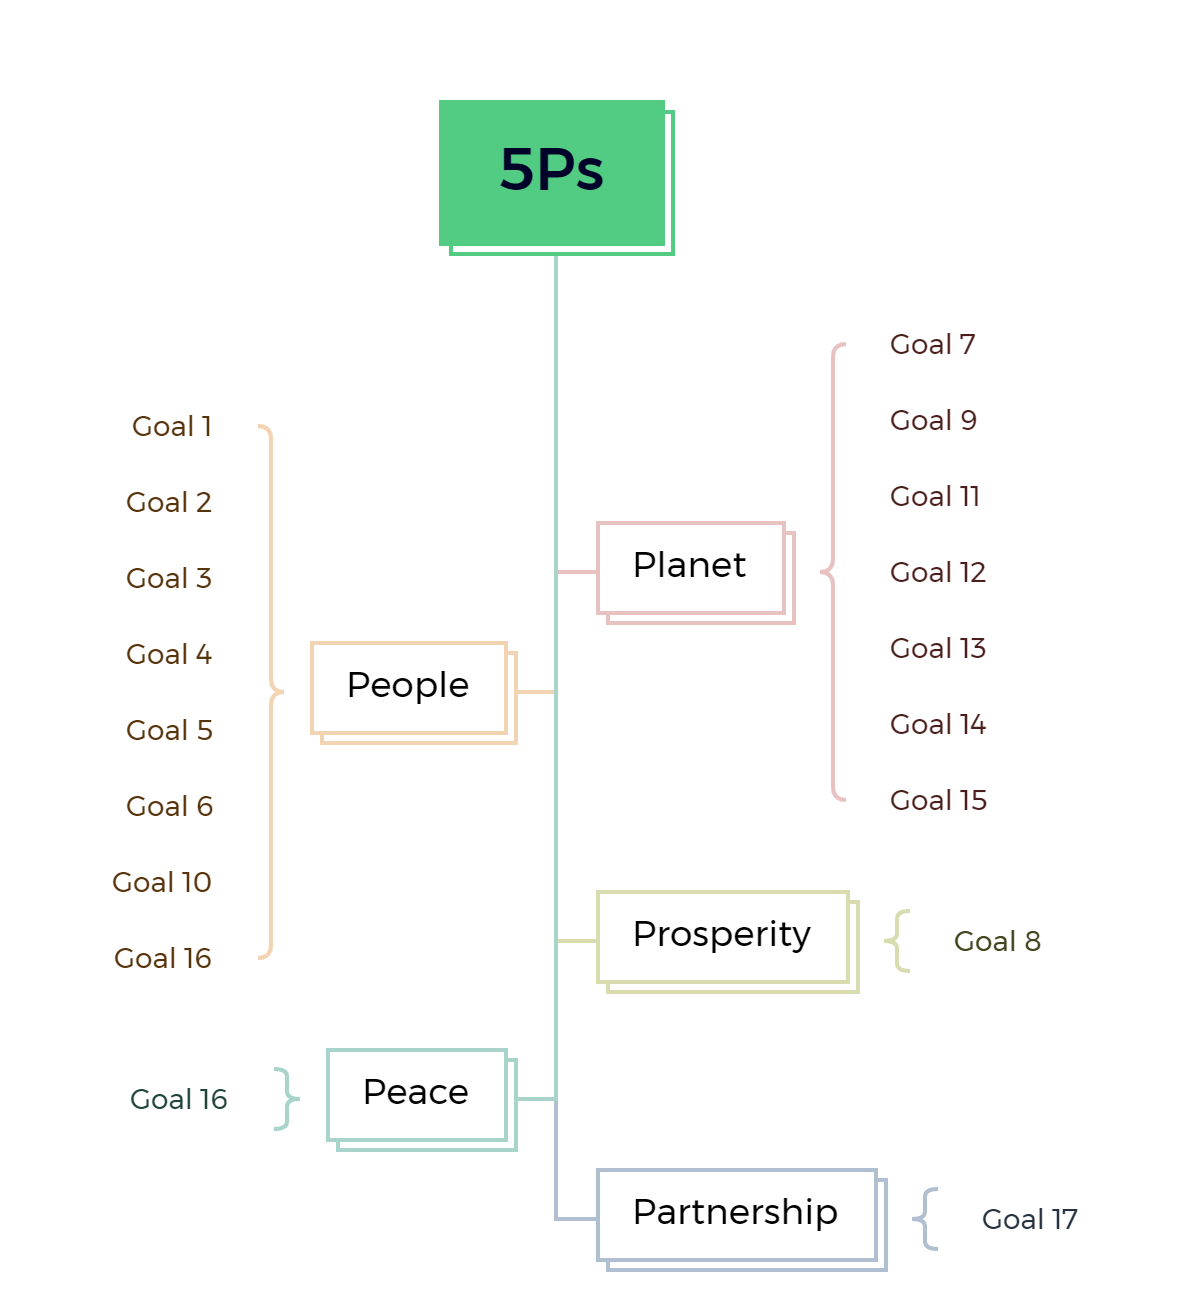
\includegraphics[scale=0.40]{{figure/5Ps-Classification.png}}%插入图片的指令
    \caption{SDGs by Categories}%标题
    \label{Label}
\end{figure}

%随后,我们根据每个可持续发展目标的关联性质,结合现实情况,理性地完成了如图所示的网络结构。
Subsequently, we rationally completed the network structure as shown in the figure, based on the nature of the association of each SDG and the reality of the situation.

\begin{figure}[h]%插入图片并且加上图片的标题,这是一个模板
    \centering
    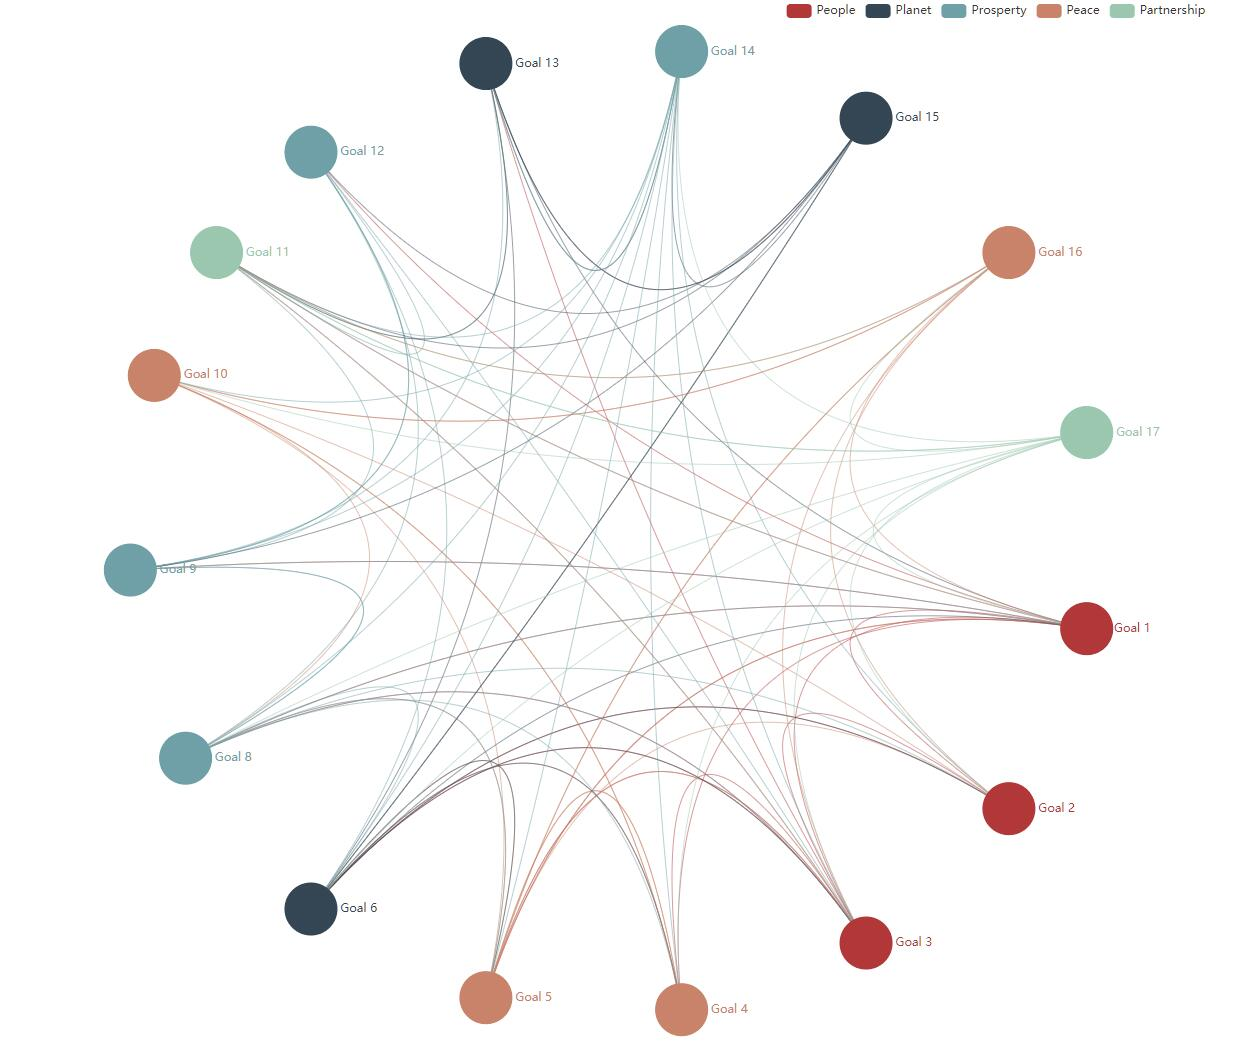
\includegraphics[scale=0.36]{{figure/Task1-Network.jpg}}%插入图片的指令
    \caption{The Network of 17 SDGs}%标题
    \label{Label}
\end{figure}

%这个关系网络非常直观地展示了具有高度相关性的议题,同时5种不同的颜色也展示了该可持续发展目标所属的主要方向和要素。两个可持续发展目标之间连线的颜色,表示了两目标之间的关系类型,了与相连曲线颜色相同的目标对所连目标具有强烈的相关影响。若两目标与连线相同,则代表具有相互影响。
This network of relationships is a very visual representation of highly relevant issues, while the five different colors show the main directions and elements to which the SDG belongs. The color of the line between two SDGs indicates the type of relationship between the two goals, and the goal with the same color as the connected curve has a strong relevant influence on the connected goal. If two goals have the same color as the connected curve, it means that they have a mutual influence.

%总之,该环形无向关系网络简单清晰地描绘了不同目标之间的归纳和作用关系。
In summary, this circular undirected relational network simply and clearly depicts the inductive and action relations between different objectives.

\section{Task2: Hierarchical Analytic Decision Model Based on AHP}

\subsection{Preparation for Model I}
%根据题目的要求,我们需要对17个可持续发展目标进行决策分析。我们将根据 Analytic Hierarchy Process (AHP) 来进行建模分析。AHP可以简便地对定性问题进行定量分析,对于抽象政策地决策问题非常有帮助。
According to the topic, we need to analyze 17 sustainable development goals for decision making. We will model the analysis based on the \textbf{Analytic Hierarchy Process} (AHP), which is an easy way to quantify qualitative problems and is useful for abstracting policy decisions.

Here is how to apply the Analytic Hierarchy Process (AHP) to the 17 Sustainable Development Goals (SDGs) that were put forward by the United Nations:

\begin{itemize}


    \item \textbf{Step 1: Define the problem and objectives}
        
    The problem is to prioritize the 17 SDGs to determine which ones are most important to focus on. The objective is to identify the most pressing SDGs that require the most attention and resources.

    \item \textbf{Step 2: Create a hierarchy}
    
    The hierarchical structure for the SDGs could look like this:
    \begin{itemize}
        \item\textbf{Goal:} Sustainable Development
        \item \textbf{Criteria:} Economic, Social, and Environmental Sustainability
        \item \textbf{Sub-criteria:} Targets of each SDG
    \end{itemize}


    \item \textbf{Step 3: Pairwise comparisons}
    
    For each level of the \textbf{hierarchy}, pairwise comparisons are made using a scale of 1 to 9. Decision-makers compare each element to every other element to determine their relative importance. For example, decision-makers might compare Economic Sustainability to Social Sustainability and Environmental Sustainability to determine their relative importance.

    \item \textbf{Step 4: Create a weight matrix}
    
    Using the results of the pairwise comparisons, a weight matrix is created for each level of the hierarchy. The weight matrix reflects the relative importance of each element. For example, the weight matrix for the criteria level might show that Economic Sustainability is more important than Social Sustainability and Environmental Sustainability.

    \item \textbf{Step 5: Evaluate the alternatives}
    
    In this case, the alternatives are the 17 SDGs. For each criterion and sub-criterion, decision-makers evaluate each SDG using a scale of 1 to 9. For example, decision-makers might evaluate SDG 1 (No Poverty) in terms of its contribution to Economic Sustainability.

    \item \textbf{Step 6: Create a score matrix}
    
    Using the results of the pairwise comparisons and the evaluations of the alternatives, a score matrix is created for each alternative. The score matrix reflects the overall desirability of each SDG. For example, the score matrix might show that SDG 13 (Climate Action) has a high overall desirability score because it contributes strongly to Environmental Sustainability.

    \item \textbf{Step 7: Check for consistency}
    
    A consistency check is performed by calculating the consistency index and consistency ratio. If the consistency ratio exceeds a pre-defined threshold, the decision-makers are required to revise their pairwise comparisons until a consistent set is obtained.
    
\end{itemize}

Once the consistency check is complete, decision-makers can use the results to prioritize the SDGs and focus their attention and resources on the most important ones. For example, the results might show that SDG 3 (Good Health and Well-Being) is the most important because it contributes strongly to all four criteria of \textbf{Economic, Social, Technological and Environmental} Sustainability.

In order to meet the requirements of Task 1, we set up Model 1, the details of which have been described in detail in Chapter 2. The ideas and methods of model setup are described here.
\\

\subsection{Establishment of Model I}
\subsubsection{Parameter Settings and Calculation about AHP}
Here we set these parameters: the discriminant matrix for comparison is \textbf{X}=$(x_{ij})_{n \times n}$, which has dimensions. 

The eigenvalues of this matrix are $\lambda$, \textbf{CI} is the consistency index, \textbf{RI} is the random consistency index, \textbf{CR} is the consistency ratio rate.

Firstly, we need to perform the calculation of relevant parameters based on Analytic Hierarchy Process (AHP). The calculation process is shown below.

\begin{itemize}
    \item \textbf{Step1: Calculate the eigenvectors of the judgment matrix}
        \begin{equation}
            \textbf{w} = \frac{\textbf{v}}{\sum_{i=1}^{n} v_i}
        \end{equation}
        
        Here, $\textbf{w}$ stands for the eigenvectors of the discriminant matrix , $\textbf{v}$ stands for the sum of column vectors of the discriminant matrix. 

\item \textbf{Step2: Calculate the Consistency Ratio (CR) of the Judgment Matrix}
\begin{equation}
\text{CR} = \frac{\lambda_{\text{max}}-n}{n-1}
\end{equation}

Here, $\lambda_{\text{max}}$ represents the maximum eigenvalue of the judgment matrix, and $n$ represents the order of the matrix.

\item\textbf{ Step3: Calculate the Maximum Eigenvalue of the Judgment Matrix}
    \begin{equation}
        \text{det}(\textbf{A}-\lambda\textbf{I}) = 0
    \end{equation}

Here, $\textbf{A}$ represents the judgment matrix, $\lambda$ represents the maximum eigenvalue, and $\textbf{I}$ represents the identity matrix.

\item \textbf{Step4: Calculate the Weight Matrix}
    \begin{equation}
        \textbf{W} = [\textbf{w}_1, \textbf{w}_2, ..., \textbf{w}_m]
    \end{equation}
Here, $\textbf{W}$ represents the weight matrix, and $\textbf{w}_i$ represents the weight vector of the $i$th layer.

\item\textbf{ Step5: Calculate the Solution Scores}
    \begin{equation}
        \textbf{S} = \textbf{W}\textbf{R}
    \end{equation}

Here, $\textbf{S}$ represents the solution score matrix, $\textbf{W}$ represents the weight matrix, and $\textbf{R}$ represents the decision matrix.

\item \textbf{Step6: Calculate the Normalized Solution Scores}
    \begin{equation}
        \textbf{N} = \frac{\sum_{i=1}^n s_i}{S}
    \end{equation}


%其中,$\textbf{N}$表示方案归一化得分矩阵,这里的$s_i$表示方案$i$在某个层次下的得分或权重。具体来说,它可以是一个准则或子准则在某个上层准则下的得分或权重,也可以是一个方案在某个准则或子准则下的得分或权重。
where $\textbf{N}$ denotes the scheme normalized score matrix, and here $s_i$ denotes the score or weight of scheme $i$ under some hierarchy. Specifically, it can be the score or weight of a criterion or sub-criterion under some upper-level criterion, or the score or weight of a scheme under some criterion or sub-criterion.

\end{itemize}

\subsubsection{Comparison of Criteria Level}
%当确定好准则和方案后,我们需要进行两个层次的比较,即准则层次的比较和方案层次的比较。这两个层次的比较都需要使用矩阵来表示,下面分别介绍。
Once the criterion and solution are determined, we need to perform two levels of comparison, namely the criterion level comparison and the solution level comparison. Both of these two levels of comparison need to be represented using matrices, which are described separately below.

%准则层次的比较:

%假设有 $n$ 个准则,我们需要确定它们之间的权重。我们可以构建一个 $n \times n$ 的矩阵 $A$,其中 $A_{ij}$ 表示准则 $i$ 相对于准则 $j$ 的重要性。由于准则 $i$ 相对于准则 $j$ 的重要性和准则 $j$ 相对于准则 $i$
Suppose there are $n$ criteria and we need to determine the weights among them. We can construct a matrix $A$ of $n \times n$, where $A_{ij}$ denotes the importance of criterion $i$ with respect to criterion $j$. Since the importance of criterion $i$ with respect to criterion $j$ and the importance of criterion $j$ with respect to the ratio of the importance of the criterion $i$ should be equal, so the matrix $A$ is a symmetric matrix, i.e., $A_{ij}=1/A_{ji}$.
%的重要性之比应该相等,因此矩阵 $A$ 是一个对称矩阵,即 $A_{ij}=1/A_{ji}$。

%我们需要使用比较刻度来衡量准则之间的重要性,比较刻度一般为 $1$ 至 $9$ 的数字,其中 $1$ 表示两个准则同等重要,$3$ 表示一个准则比另一个准则稍微重要一些,$5$ 表示一个准则比另一个准则明显重要,$7$ 表示一个准则比另一个准则非常重要,$9$ 表示一个准则比另一个准则绝对重要。
We need to measure the importance between criteria using a \textbf{comparison scale}, which is generally a number from $1$ to $9$, where $1$ means that both criteria are equally important, $3$ means that one criterion is slightly more important than the other, $5$ means that one criterion is significantly more important than the other, $7$ means that one criterion is very important than the other, and $9$ means that one criterion is absolutely more important than the other.

%为了确定矩阵 $A$,我们需要让用户对每对准则进行两两比较,得到比较刻度 $a_{ij}$,然后根据下面的公式计算 $A_{ij}$:
In order to determine the matrix $A$, we need to let the user make a two-by-two comparison for each pair of criteria to obtain the comparison scale $a_{ij}$ and then calculate $A_{ij}$ according to the following formula.

\begin{equation}
   A_{ij}=\begin{cases}1 & i=j\\\alpha_{ij} & i \neq j\end{cases}
\end{equation}


%例如,假设我们有三个准则:环保、经济效益和社会效益,我们需要让用户对它们进行两两比较。如果用户认为环保比经济效益稍微重要一些,比社会效益明显重要一些,那么比较刻度为 $3$ 和 $5$。因此,我们可以计算出矩阵 $A$ 如下:
For example, suppose we have five criteria: \textbf{Importance, Achievability, Urgency, Time Horizon and Alignment}.We need to ask users to compare them two by two. If the user thinks that urgency is slightly more important than importance and significantly more important than social benefits, then the comparison scales are $3$ and $5$. Thus, we can calculate the matrix $A$ as follows.

\subsubsection{Comparison of Alternative Level and Development}
%方案层次的比较:

%假设有 $m$ 个方案,我们需要确定它们之间的权重。我们可以构建一个 $n \times m$ 的矩阵 $B$,其中 $B_{ij}$ 表示准则 $i$ 对方案 $j$ 的重要性。
Suppose there are $m$ scenarios and we need to determine the weights among them. We can construct a matrix $B$ of $n \times m$, where $B_{ij}$ denotes the importance of criterion $i$ to scheme $j$.

%同样,我们需要使用比较刻度来衡量准则对方案
Similarly, we need to use a comparison scale to measure the effect of the criterion on the program

%下面是hwq写的,等会融合一下:

%下面,我来对层次分析法进行描述,并结合该问题进行建模。
In the following, I will describe the hierarchical analysis method and model it in the context of the problem.


%层次分析法分为三个部分,分别是上层中层和下层。中层是决策层,下层是方案层。决策层分为不同的核心决策要点,每一个方案都和决策层相关,这样的话上层和下层都分别和决策层有一个“比较判别矩阵”: 
\textbf{Hierarchical analysis} is divided into three parts, which are the upper middle level and the lower level. The middle level is the decision level and the lower level is the solution level. The decision level is divided into different core decision points and each solution is related to the decision level, so that the upper and lower levels have a "comparative discriminant matrix" with the decision level respectively. 

\begin{equation}
\mathbf{X} =(x_{ij})_{n \times n} 
\end{equation}
where n represents the number of various decision indicators or solutions in the middle or lower level, and $x_{ij}$ denotes the relative importance of each $i$ element with respect to the quantification of the $j$th element with respect to some indicator in the upper level, where the element $x_{ii}=1,i=1,...,n$ located on the diagonal; for the elements in the matrix, the following conditions need to be satisfied:



     $$x_{ij}>0,
     x_{ij}  = \frac{1}{x_{ji}},
     x_{ii} = 1,
     i,j\in\{1,...,n\}$$





We need to decide the weight proportion of the decision level through discussion and analysis, and we refer to relevant papers in this regard.


The results are shown below:
\begin{center}
    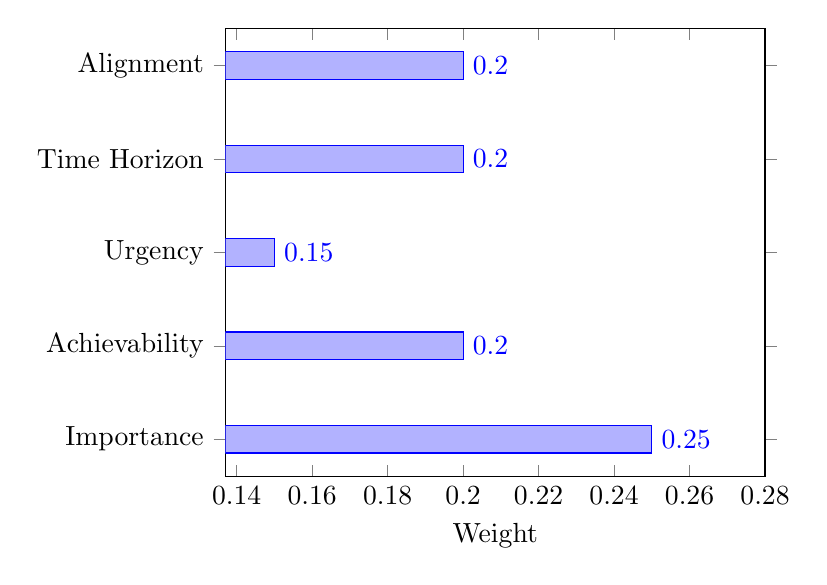
\begin{tikzpicture}
    \begin{axis}[
        xbar,
        xlabel={Weight},
        symbolic y coords={Importance,Achievability,Urgency,Time Horizon,Alignment},
        ytick=data,
        xmax=0.28,
        nodes near coords,
        nodes near coords align={horizontal},
        ]
    \addplot coordinates {
        (0.25,Importance)
        (0.20,Achievability)
        (0.15,Urgency)
        (0.20,Time Horizon)
        (0.20,Alignment)};
    \end{axis}
\end{tikzpicture}
\end{center}

For this weight icon, we conclude, based on the consistency test, that the icon is consistent with the relevant logic and has some scientific reference value.
%对于这张权重图标,我们根据一致性检验,得出,该图标符合相关逻辑,并具有一定的科学参考价值。

Next, we provide an in-depth analysis of the relevant content.
%接下来,我们对相关内容进行深度分析。

According to the theory of AHP, we can get the final weight ratios of each decision by solving the characteristic roots of the weight matrix. Subsequently, we need to discuss the corresponding \textbf{weight ratios} for each solution, in a certain characteristic, so that we can calculate the weight analysis relationship for each solution, and thus get the final weight relationship for each objective. Due to the large content of the correlation matrix, we list it in the final code section. Below are the final values of the weight relationships between the different sustainable development goals that we obtained.
%根据AHP的理论,我们通过求解权重矩阵的特征根,可以得到最后的各个决策的权重占比。随后我们需要讨论每一个方案,在某个特性中的对应权重比值,从而可以计算出各个方案的权重分析关系,从而得到最后每一个目标的权重关系。由于相关矩阵内容较多,我们将其列在最后的代码部分之中。下方为我们最终求得的不同可持续发展目标之间的权重关系值。

\begin{figure}[h]
    \centering
    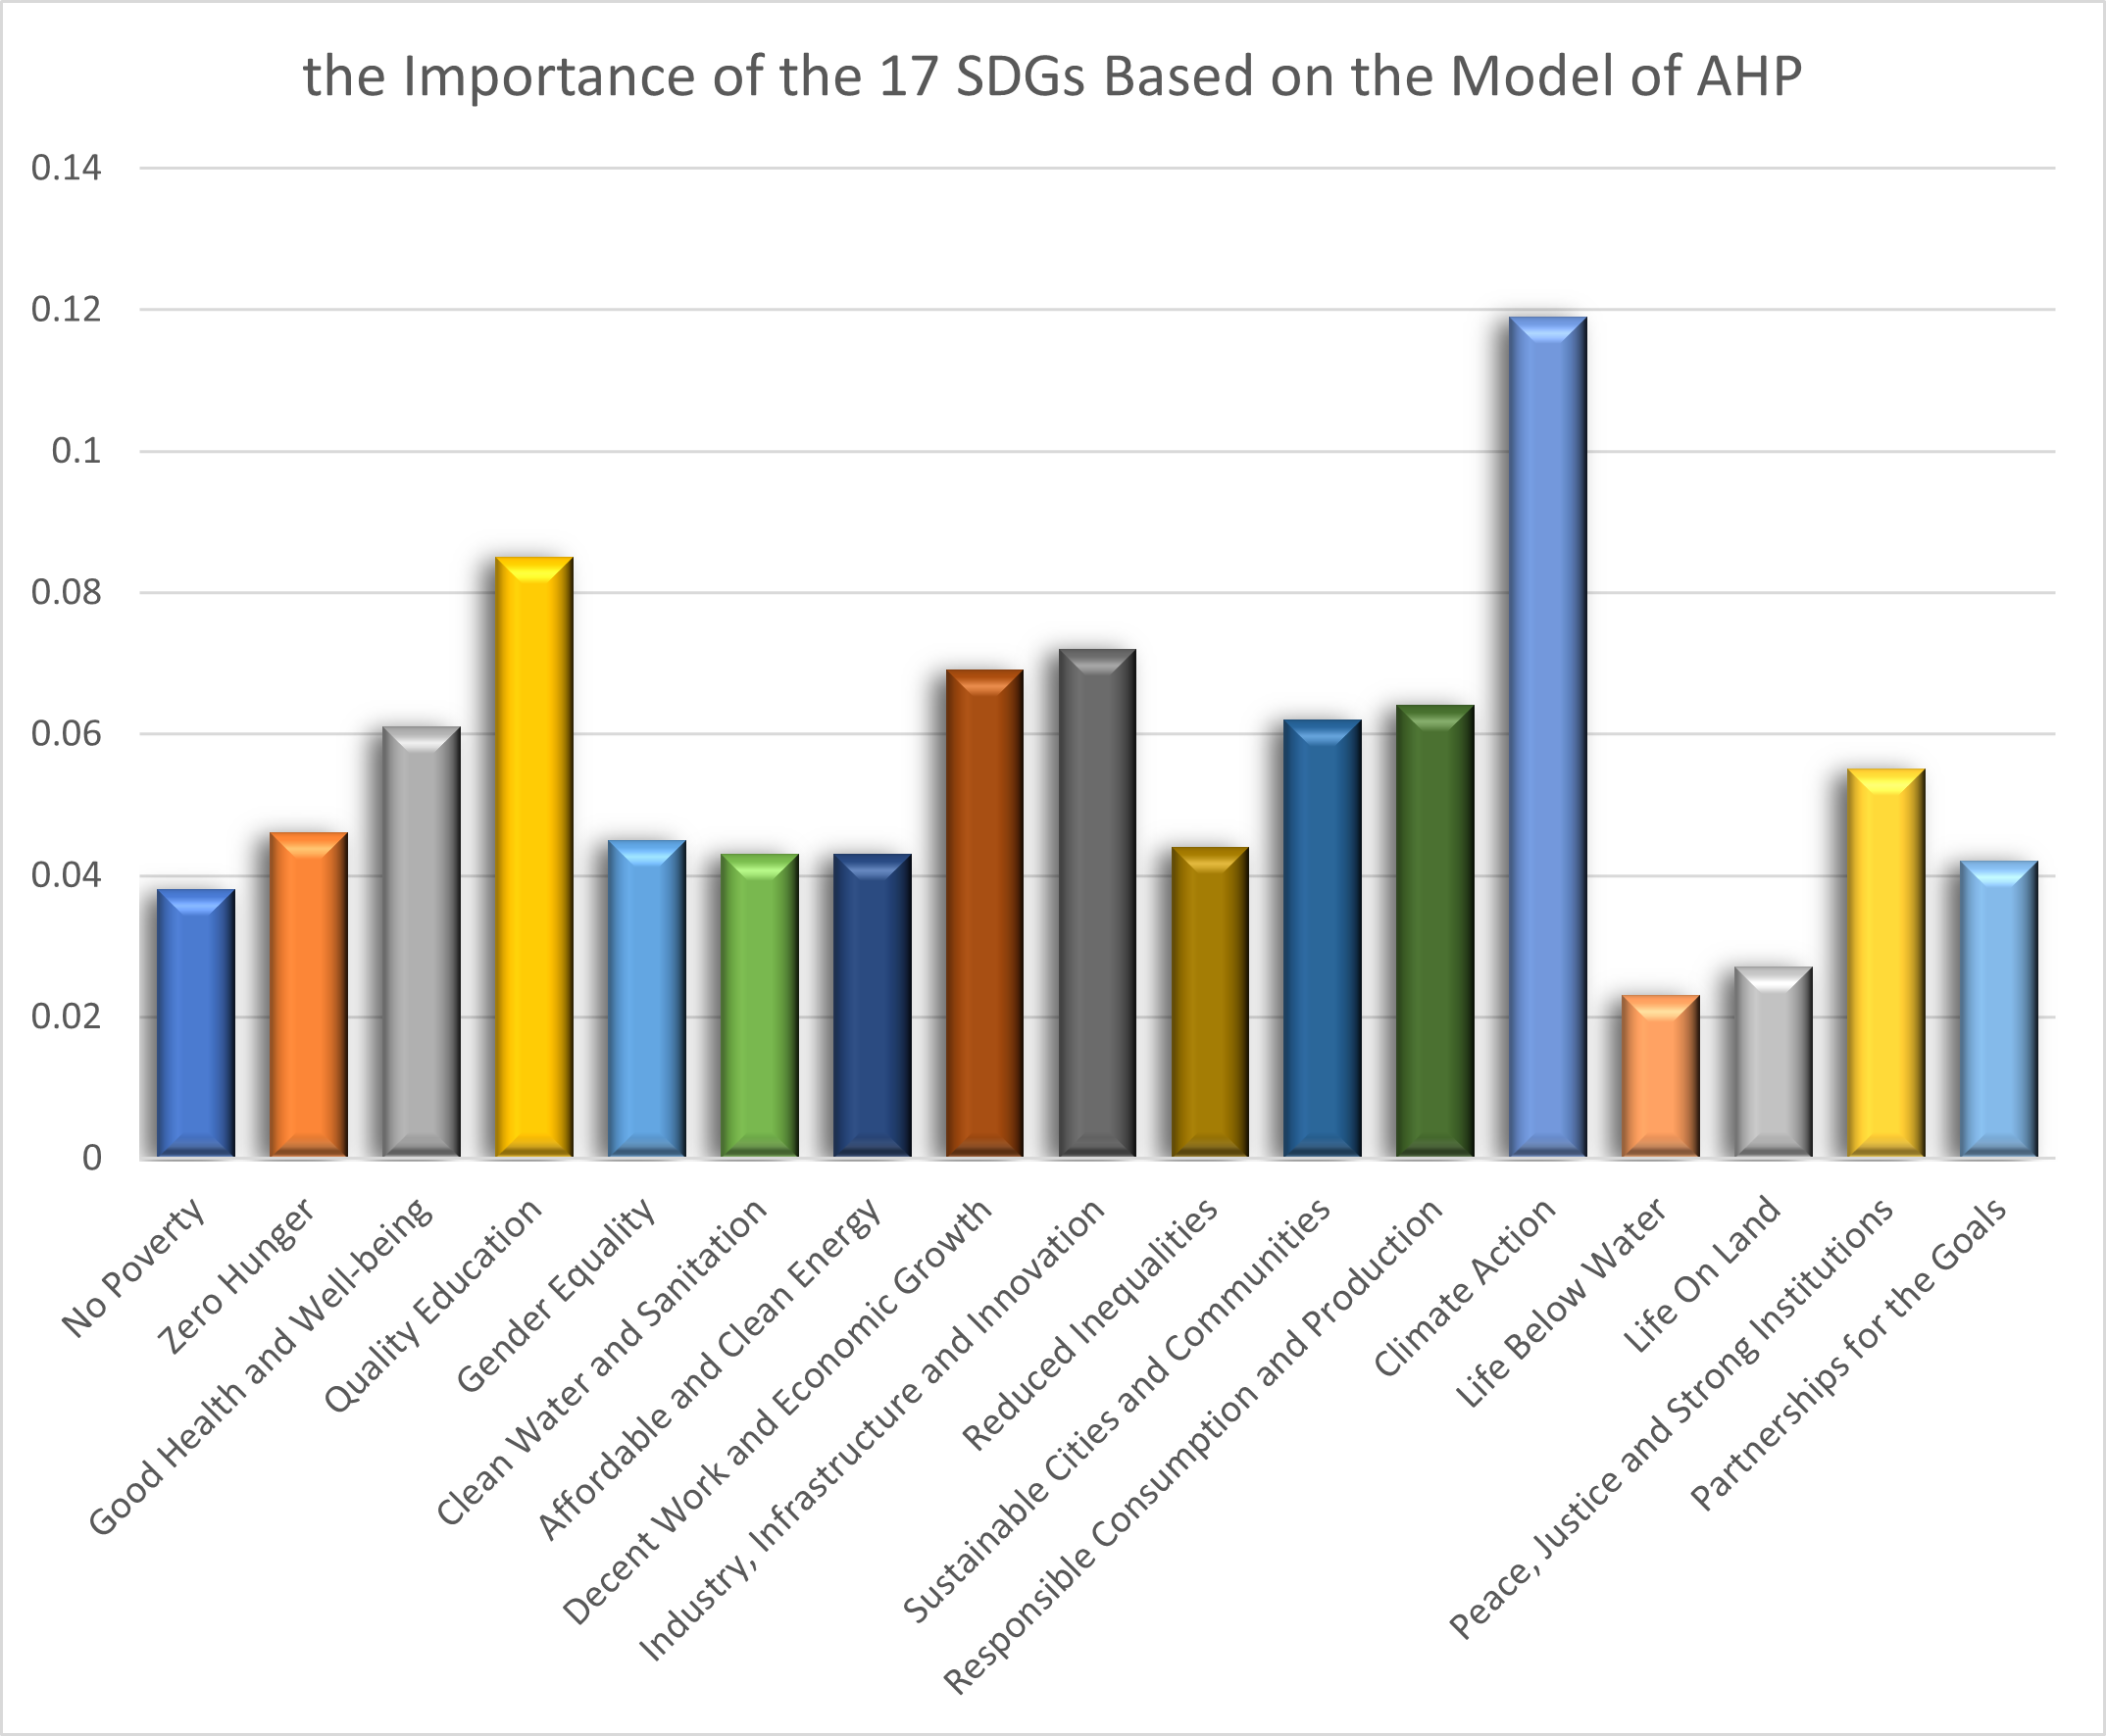
\includegraphics[scale=0.6]{{figure/the_Importance_of_the_17_SDGs_Based_on_the_Model_of_AHP.png}}%插入图片的指令
    \caption{the Importance of the 17 SDGs Based on the Model of AHP}%标题
    \label{Label}
\end{figure}

Looking at the data, we can see that SDG 13, Climate Action, has the highest priority value for this item, so Goal 13 has the highest priority.
%观察数据可以看到,可持续发展目标13,Climate Action这一项优先级数值最高,因此目标13优先级最高。

Climate Action is a broad topic that typically refers to a variety of measures taken to address climate change. These measures can be divided into the following categories.
%Climate Action是一个广泛的主题,通常指为应对气候变化而采取的各种措施。这些措施可以分为以下几类:

\begin{itemize}
\item \textbf{Reduce greenhouse gas emissions:} Reduce greenhouse gas emissions: This is one of the most basic measures to combat climate change. By using clean energy, improving energy efficiency, and promoting low-carbon travel patterns, we can reduce greenhouse gas emissions such as carbon dioxide and methane.
%减少温室气体排放: 减少温室气体排放:这是最基本的应对气候变化的措施之一。通过使用清洁能源、提高能源效率、推广低碳出行方式等,减少二氧化碳、甲烷等温室气体的排放。

\item \textbf{Adaptation to Climate Change:} Adaptation to climate change has become an important task as climate change is already causing a range of impacts, such as extreme weather events and sea level rise. Measures to adapt to climate change include building healthier and safer cities, protecting ecosystems, and reducing risks.
%适应气候变化: 由于气候变化已经带来了一系列的影响,如极端气候事件、海平面上升等,适应气候变化也成为了一项重要的任务。适应气候变化的措施包括建立更健康、更安全的城市、保护生态系统、减少风险等。

\item \textbf{Transition to a sustainable development model:} Since existing development models often come at the expense of the environment, a transition to a sustainable development model becomes a must. This includes an economic model that values environmental protection, efficient resource use, and encourages innovation and investment in sustainability.
%转型到可持续发展模式: 由于现有的发展模式往往是以牺牲环境为代价的,转型到可持续发展模式成为了必须的选择。这包括了重视环境保护、资源利用的高效率、以及鼓励创新和投资可持续性的经济模式。

\item \textbf{Climate Awareness:} While more and more people are recognizing the seriousness of climate change, there is still a need to increase global public awareness and understanding of climate change in order to better contribute to it.
%提高气候意识: 尽管越来越多的人已经认识到气候变化的严重性,但仍然需要提高全球公众对气候变化的意识和理解,以便更好地为气候变化做出贡献。
\end{itemize}

Climate Action covers many areas, including energy, urban planning, transportation, agriculture, water management, etc., and the measures taken should be diverse.\\
%Climate Action的内容涉及了许多领域,包括能源、城市规划、交通、农业、水资源管理等,而采取的措施也应该是多样化的。


If the \textbf{implementation of climate action} is initiated as a priority, the following objectives can be achieved.
%如果优先启动实施气候行动,可以实现以下目标:

\begin{itemize}
\item \textbf{Reducing greenhouse gas emissions:} Carbon emissions can be reduced and global warming slowed by promoting renewable energy and clean energy technologies, and by enhancing energy efficiency.
%减少温室气体排放:通过推广可再生能源和清洁能源技术,以及加强能源效率,可以减少碳排放量并减缓全球变暖。
\item \textbf{Protecting ecosystems:} By promoting sustainable development and conservation measures, we can mitigate the effects of climate change and promote the restoration and protection of ecosystems.
%保护生态系统:通过推动可持续发展和采取保护措施,可以减缓气候变化带来的影响,并促进生态系统的恢复和保护。
\item \textbf{Promoting sustainable economic development:} By investing in renewable energy and other green technologies, new jobs and economic growth can be created, driving sustainable economic development.
%促进可持续经济发展:通过投资于可再生能源和其他绿色技术,可以创造新的就业机会和经济增长,推动可持续经济发展。
\item \textbf{Raising public awareness:} Through education and publicity, public awareness of climate change and environmental protection can be raised, action and cooperation can be promoted, and the awareness and action of the whole society to tackle climate change together can be formed.
%提高公众意识:通过教育和宣传,可以提高公众对气候变化和环境保护的意识,促进行动和合作,形成全社会共同应对气候变化的意识和行动。
\end{itemize}

\textbf{In conclusion,} implementing climate action can promote sustainable social and economic development, mitigate the effects of climate change, and increase public awareness and attention to environmental protection, leading to a cleaner, greener, healthier and more sustainable lifestyle for the next decade.
%总之,实施气候行动可以推动社会和经济的可持续发展,减缓气候变化的影响,并提高公众对环境保护的意识和重视程度,为未来10年带来更加清洁、绿色、健康和可持续的生活方式。
%%%%%%%%%%%%%%%%%%%%%%%%%%%%%%%%%%%%%%%%%%%%%%%%%

\section{Task 3: Hierarchical Clustering Decision Model based on AHP and K-Means}%基于 AHP 和 K-Means 的群体分析决策模型
\subsection{Cluster Optimization based on Model I}
The AHP model we have just built is a good representation of the most important target decisions we need to make, but it has the obvious drawback that our model requires a lot of data and a lot of work to process the data. This model is not perfect in terms of ease of use and simplicity. Therefore, we have improved the AHP model, especially to enhance its ease of use and computational simplicity.
%我们刚刚建立的AHP模型可以很完好的展示计算我们最需要的目标决策,但是这个模型也有着很明显的缺陷,那就是我们的模型需要非常繁杂的数据,同时也有着非常麻烦的数据处理工作。从易用性和简便性的角度考虑,这个模型都不算非常完善。因此我们对AHP模型进行了完善的处理,尤其用来增强其易用性和计算的简便性。

The refinement of the model has two parts:
%模型的完善有两个部分:
\begin{itemize}
    \item \textbf{On the one hand,} we have changed the overall data processing process and added a data pre-processing process to facilitate better and more complete classification of the data in the end and to perform the final calculations.
    %一个是我们更改了整体的数据处理流程,增加了数据预处理的流程,以便于最终更好更完善地将数据进行分类,并进行最终的计算。
    \item \textbf{On the other hand,} we optimized the pre-processing content of the model for better simplification of the data.
    %另一方面我们优化了模型的预处理内容,以便于更好的进行数据的简便化处理。
\end{itemize}\\

Our optimizations are as follows.
\begin{itemize}
    \item \textbf{Step1:} We use the 5Ps as the evaluation criteria for the 17 goals, and each goal will be scored from 0-100 based on these 5 evaluation indicators, which in turn leads to a scoring matrix composed of 17 goals %首先,我们将5Ps作为17个目标的评价标准,每个目标会根据这5个评价指标进行0-100的打分,进而得到17个目标构成的评分矩阵
    $\mathbf{X}=[x_1,x_2,...,x_n]$, Then each target will have a score vector for these 5 criteria
    %那么每个目标对于这5个标准就会有一个评分向量
    \begin{equation}
        x_i=(x_{i1},x_{i2},x_{i3},x_{i4},x_{i5}),i=1,...,17,x_{ij}\in{0,...,100}
    \end{equation}
    A vector representing the score assigned to the ith goal under the People, Planet, Prosperity, Peace, Partnership evaluation metric.%代表第i个目标在People,Planet,Prosperity,Peace,Partnership评价指标下被赋予的评分的向量。
    
    \item \textbf{Step2:} Then the 17 targets are classified into N classes by K-means clustering algorithm with 5 evaluation metrics as features. Also, because the K-means algorithm classification has uncertainty, we need to use this algorithm several times in this dataset and choose the one with the smallest loss function among multiple results as our final classification.  %Step2: 然后通过K-means聚类算法,以5个评价指标为特征,将17个目标分成N类。同时因为K-means算法分类具有不确定性,因此我们需要多次在这个数据集中使用这个算法,在多个结果中选择损失函数最小的那个分类作为我们的最终分类。  
    
    \item \textbf{Step3:} The objectives in each class are put into the solution layer of AHP separately by class, so that the relatively more important one in these classes can be solved by AHP, and then the most important one in each class is taken out and put into AHP again for solving, so that the second optimal solution after a certain objective is completed can be calculated. %最后,分别将各个类中的目标分别按类放进AHP的方案层,这样可以通过AHP求解出这些类中相对比较重要的某一项,然后将每一类中最重要的一项取出,再次放进AHP中进行求解,这样子就可以算出完成了某一目标后的第二个最优方案。
\end{itemize}

\subsection{Preparing and Parameter Setting for Model II}



First, the 17 scenarios are represented as 17 points in the feature space, each point representing a scenario, and the dimension of the feature space is chosen as needed. For AHP, each scheme corresponds to multiple criteria/factors, and each criterion/factor can be used as a dimension of the feature space. While for \textbf{K-Means}, each scheme may have only one or several numerical indicators as features, and each indicator can be used as one dimension of the feature space.
%首先,将17个方案表示成特征空间中的17个点,每个点代表一个方案,特征空间的维度根据需要选择。对于AHP,每个方案对应着多个标准/因素,可以将每个标准/因素作为特征空间的一个维度。而对于K-Means,每个方案可能只有一个或者几个数值型指标作为特征,可以将每个指标作为特征空间的一个维度。

These points are then clustered into several groups using the K-Means algorithm. the basic idea of the K-Means algorithm is to randomly select k initial clustering centers and then attribute each point to the cluster of its nearest clustering center. Then the centers of each cluster are recalculated and each point is reattributed to the cluster of its nearest cluster center, and so on iteratively until the cluster centers no longer change or the preset number of iterations is reached
%然后,利用K-Means算法将这些点聚类成若干个群体。K-Means算法的基本思想是随机选择k个初始聚类中心,然后将每个点归属到离其最近的聚类中心的聚类中。然后重新计算每个聚类的中心,并将每个点重新归属到距离其最近的聚类中心的聚类中,如此循环迭代直到聚类中心不再发生变化或达到预设迭代次数。


For each cluster, AHP is used to further analyze it for decision making. For each cluster, it can be considered as a whole for AHP's hierarchy building and judgment matrix construction. In the judgment matrix, for the solutions in the same cluster, the relative importance between them is determined by the AHP method. Eventually, the weighted score of each cluster can be obtained, indicating the relative merits of the solutions represented by that cluster.%对于每个聚类,使用AHP对其进行进一步的决策分析。对于每个聚类,可以将其视为一个整体进行AHP的层次结构建立和判断矩阵的构造。在判断矩阵中,对于同一聚类中的方案,它们之间的相对重要性由AHP方法决定。最终,可以得到每个聚类的加权得分,表示该聚类代表的方案的相对优劣。

Finally, the weighted scores of all clusters are considered together, and the cluster with the highest score and the solution in it are selected as the final decision solution.%最后,综合考虑所有聚类的加权得分,选择得分最高的聚类及其中的方案作为最终的决策方案。




\begin{figure}[h]
    \centering
    \begin{minipage}[t]{0.4\linewidth}
        \centering
        \begin{cases}
        \lambda_{max} = \frac{\textbf{w}^T\textbf{A}\textbf{w}}      {\textbf{w}^T\textbf{w}}\\
          CI = \frac{\lambda_{max} - n}{n - 1}\\
         CR = \frac{CI}{RI}\\
         w_i = \frac{\prod_{j=1}^n a_{ij}^{1/n}} {\sum_{i=1}^n\prod_{j=1}^n a_{ij}^{1/n}} \\
        \textbf{w} = (w_1, w_2, ..., w_n)\\
\end{cases}
    \end{minipage}%
    \begin{minipage}[t]{0.4\linewidth}
        \centering
        $\begin{array}{@{}l@{}}
            RI = \begin{cases}
                0, &n=1\\
                1, &n=2\\
                \frac{0.58(n-2)}{n-1}+1, &n\geq3
            \end{cases} 
        \end{array}$
    \end{minipage}
    \caption{Analytic Hierarchy Process (AHP) Parameters Setting}
    \label{fig:ahp}
\end{figure}



The parameters of this model are similar to those of model 1 and will not be repeated here.%该模型的参数与模型1相似,在此处不再赘述。


\subsection{Establishment of Model II:}

Suppose there are $n$ schemes and each scheme $i$ is represented by $m$ indicators, we consider each scheme as a point $\boldsymbol{x_i}=(x_{i1},x_{i2},\cdots,x_{im})$ in $m$-dimensional space, where $x_{ij}$ denotes the value of scheme $i$ on the $j$th indicator.
%假设有 $n$ 个方案,每个方案 $i$ 由 $m$ 个指标表示,我们将每个方案视为 $m$ 维空间中的一个点 $\boldsymbol{x_i}=(x_{i1},x_{i2},\cdots,x_{im})$,其中 $x_{ij}$ 表示方案 $i$ 在第 $j$ 个指标上的取值。

First, these points are clustered into $k$ groups using the k-means algorithm to obtain the clustering center of each group $\boldsymbol{c_j}=(c_{j1},c_{j2},\cdots,c_{jm})$, where $j\in{1,2,\cdots,k}$. The clustering centers are calculated as follows.
%首先,使用 k-means 算法将这些点聚类成 $k$ 个群体,得到每个群体的聚类中心 $\boldsymbol{c_j}=(c_{j1},c_{j2},\cdots,c_{jm})$,其中 $j\in{1,2,\cdots,k}$。聚类中心的计算公式如下:

We use the following equation to calculate the centroid $c_j$ of the $j$th cluster:

\begin{equation}
c_j = \frac{1}{n_j} \sum\limits_{i=1}^{n} x_i \cdot I(y_i=j)
\end{equation}

Here, $n_j$ represents the number of samples in the $j$th cluster, and $\mathbb{I}(\cdot)$ is an indicator function that takes the value of 1 when $y_i=j$ and 0 otherwise. Initially, we can randomly select $k$ points as the initial clustering centers.

Next, for each cluster $j$, we use AHP for further decision analysis. Firstly, we construct the hierarchy of AHP based on the schemes in the cluster and obtain the judgment matrix $\boldsymbol{A_j}$. In the judgment matrix, the relative importance among the schemes in the same cluster is determined by the AHP method.

The calculation steps are as follows:

\begin{itemize}
\item[1] \textbf{Construct} the judgment matrix $\boldsymbol{B}$, where $b_{ij}$ represents the importance of scheme $i$ relative to scheme $j$, which can be determined by experts or subjective evaluation. The judgment matrix should satisfy the positive reciprocal property, i.e.,
    \begin{equation}
        b_{ij}=1/b_{ji}
    \end{equation}

\item[2] \textbf{Normalize} the judgment matrix to obtain the weight vector $\boldsymbol{w}=(w_1,w_2,\cdots,w_n)$, where $w_i$ represents the weight of scheme $i$.

    \begin{equation}
        w_i = \sum_{k=1}^n \left(\prod_{j=1}^n b_{kj}^{1/n}\right)\left(\prod_{j=1}^n b_{ij}^{1/n}\right)
    \end{equation}

\item[3] \textbf{Calculate} the weighted score $s_{ij}$ of each scheme in the cluster, which represents the relative importance of scheme $i$ in cluster $j$.

    \begin{equation}
        s_{ij} = \sum\limits_{k=1}^{n_j} w_k \cdot w_i
    \end{equation}
\end{itemize}

We have illustrated the \textbf{Framework Diagram} below.





\begin{figure}[h]
    \centering
    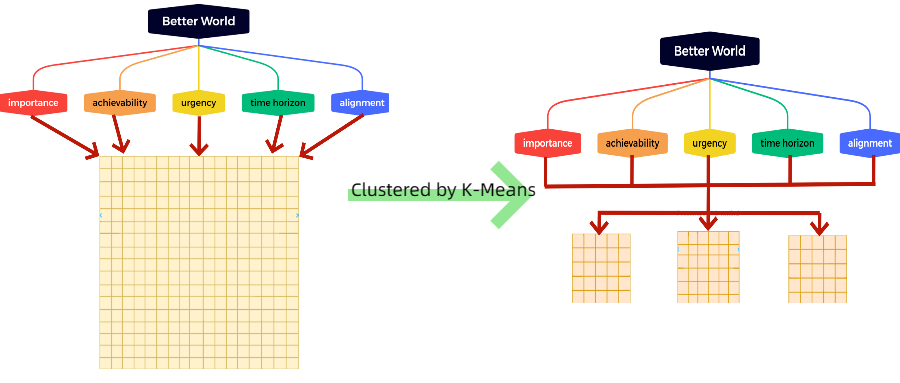
\includegraphics[scale=0.49]{{figure/Matrix_Change.png}}%插入图片的指令
    \caption{The Change of AHP After the Goals Clustered by K-Means}%标题
    \label{Label}
\end{figure}

\newpage

\subsection{Application for Model II}
According to the flowchart, we used K-means algorithm to preprocess the data and then used AHP to calculate the final weight proportions.
After clustering the 17 sustainable development goals with K-means, we obtained K=3, and the clustering results are as follows:

\begin{table}[htbp]
\centering
\caption{Clusters of Sustainable Development Goals}
\begin{tabular}{cccc}
\toprule
\textbf{Cluster 1} & \multicolumn{3}{c}{2, 3, 4, 5, 6, 7, 8, 9, 10, 11, 15} \\
\midrule
\textbf{Cluster 2} & \multicolumn{3}{c}{1, 16, 17} \\
\midrule
\textbf{Cluster 3} & \multicolumn{3}{c}{12, 13, 14} \\
\bottomrule
\end{tabular}%
\label{tab:clusters}%
\end{table}






Based on the K-means clustering and subsequent AHP calculation, we can divide the 17 sustainable development goals into four categories, each containing the goals from the respective clusters. Then, we can calculate the weights for each category using AHP, resulting in the following:

\begin{itemize}

\item \textbf{Cluster 1:} Sustainability goal 
\item \textbf{Cluster 2:} Infrastructure and inequality goals
\item \textbf{Cluster 3:} Education and health goals
\end{itemize}

    \begin{table}[htbp]
    \centering
    \caption{Weights for Goal Clusters}
    \begin{tabular}{|c|c|}
    \hline
    \textbf{Goal Cluster} & \textbf{Weight} \\
    \hline
    Social sustainability goals & 0.479 \\
    \hline
    Economic sustainability goals & 0.319 \\
    \hline
    Environmental sustainability goals & 0.202 \\
    \hline
    Infrastructure goals & 0.556 \\
    \hline
    Inequality goals & 0.444 \\
    \hline
    Education goals & 0.560 \\
    \hline
    Health goals & 0.440 \\
    \hline
    \end{tabular}
    \label{tab:my_table}
    \end{table}


\begin{figure}[h]
    \centering
    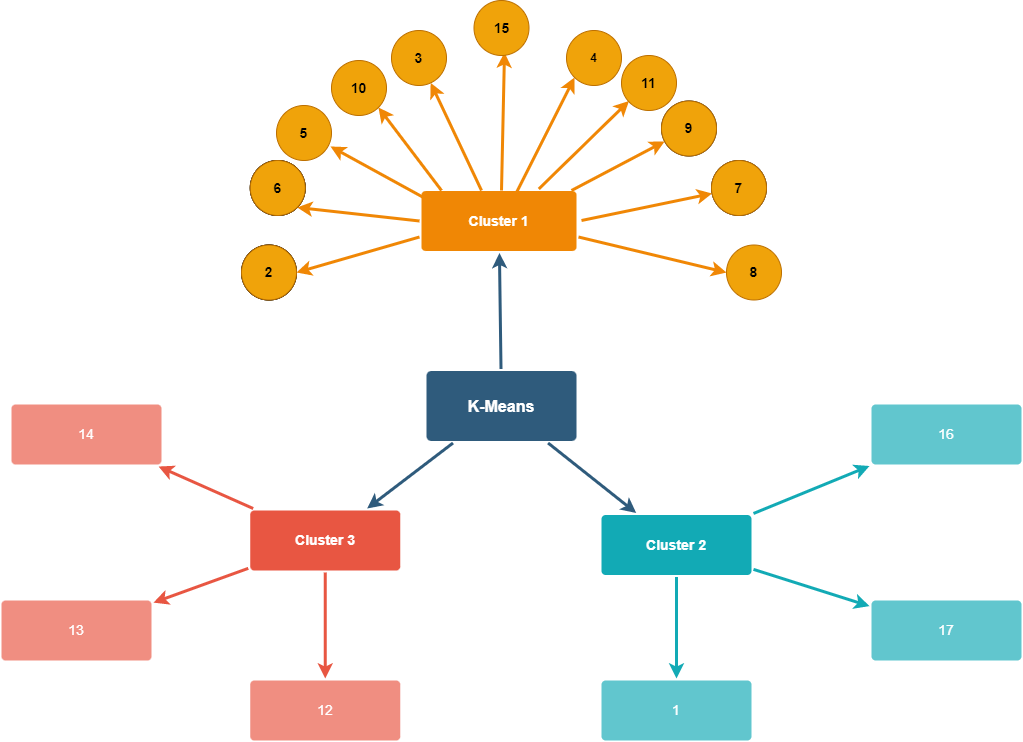
\includegraphics[scale=0.35]{{figure/K-means.png}}%插入图片的指令
    \caption{Clusters Divided by K-Means}%标题
    \label{Label}
\end{figure}

Therefore, the weights for the 17 sustainable development goals are as follows.

Assuming there is no hunger, we have conducted K-means clustering on the 17 sustainable development goals based on the evaluation matrix 
\begin{equation}
    \mathbf{X}=[\mathbf{x_1},\mathbf{x_2},\dots,\mathbf{x_n}]
\end{equation}
where $\mathbf{x_i}=(x_{i1},x_{i2},x_{i3},x_{i4},x_{i5}),i=1,\dots,17,x_{ij}\in{0,\dots,100}$ represents the score vector of the $i$th goal in the People, Planet, Prosperity, Peace, Partnership dimensions.

Next, we use the AHP method to calculate the weights of each sustainable development goal in the five dimensions. Let $\mathbf{w}=(w_1,w_2,w_3,w_4,w_5)$ be the weight vector, and the specific values are as follows:

\begin{equation}
   \mathbf{w}=(0.176,0.192,0.281,0.099,0.253)
\end{equation}

and finally, the weights of Importance,Achievability,Urgency,Time Horizon,Alignment are 0.176, 0.192, 0.281, 0.099, and 0.253, respectively.

After calculation, in the absence of hunger, the weights of the 17 sustainable development goals are:





\begin{comment}

\begin{table}[htbp]
\centering
\caption{Weights for each Sustainable Development Goal}
\begin{tabular}{|c|c|c|}
\hline
\textbf{Sustainable Development Goal} & \textbf{Weight with no Poverty} & \textbf{Weight with no Hunger} \\
\hline
No Poverty & 0.059 & 0.066 \\
\hline
Zero Hunger & 0.058 & 0.072 \\
\hline
Good Health and Well-being & 0.062 & 0.072 \\
\hline
Quality Education & 0.063 & 0.077 \\
\hline
Gender Equality & 0.058 & 0.072 \\
\hline
Clean Water and Sanitation & 0.055 & 0.069 \\
\hline
Affordable and Clean Energy & 0.049 & 0.062 \\
\hline
Decent Work and Economic Growth & 0.056 & 0.071 \\
\hline
Industry, Innovation and Infrastructure & 0.056 & 0.071 \\
\hline
Reduced Inequalities & 0.054 & 0.068 \\
\hline
Sustainable Cities and Communities & 0.055 & 0.068 \\
\hline
Responsible Consumption and Production & 0.054 & 0.067 \\
\hline
Climate Action & 0.062 & 0.077 \\
\hline
Life Below Water & 0.057 & 0.071 \\
\hline
Life On Land & 0.060 & 0.074 \\
\hline
Peace, Justice and Strong Institutions & 0.057 & 0.070 \\
\hline
Partnerships for the Goals & 0.056 & 0.069 \\
\hline
\end{tabular}%
\label{tab:sdg_weights_combined}%
\end{table}

\end{comment}

\begin{figure}[h]
    \centering
    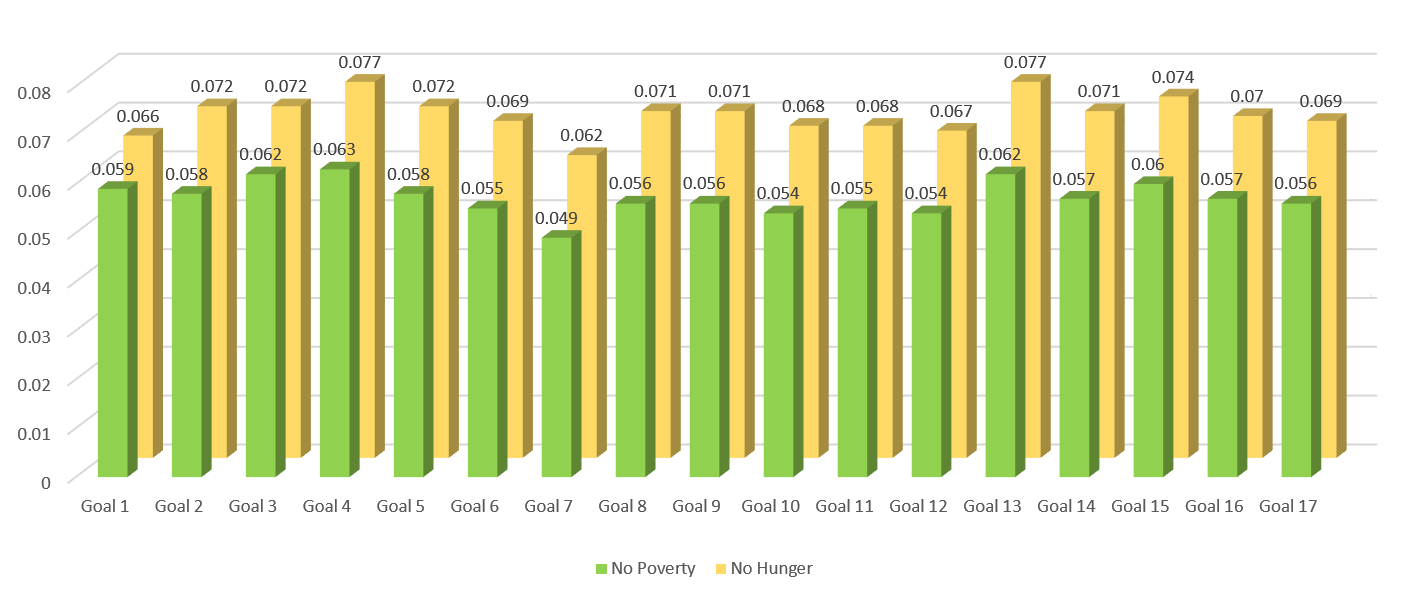
\includegraphics[scale=0.66]{{figure/Weight_2Ns.png}}%插入图片的指令
    \caption{Weights for No Poverty and 
 No Hunger}%标题
    \label{Label}
\end{figure}
According to the results, quality education and climate action should be the first priorities to promote sustainable development in a hunger-free world.

Similarly, when there is no poverty, the weight values for Importance, Achievability, Urgency, Time Horizon, and Alignment are 0.180, 0.197, 0.289, 0.101, and 0.233 respectively.

Some weights of the 17 sustainable development goals are:
\begin{itemize}
    \item \textbf{No Hunger}: 0.065
    \item \textbf{Good Health and Well-being}: 0.064
    \item \textbf{Quality Education}: 0.066
\end{itemize}



When poverty is eradicated, it becomes crucial to prioritize quality education in order to ensure technological progress and civilized development, which in turn can promote sustainable development. Quality education provides individuals with the knowledge and skills needed to actively participate in the workforce, innovate new technologies, and make informed decisions about their lives and communities. This can lead to a more sustainable and equitable society, with improved health, reduced inequality, and increased economic growth.

More detailed information can be found in the bar chart below. The chart provides a clear view of the weights assigned to different goals, as well as their comparisons and trends over time.



%%%%%%%%%%%%%%%%%%%%%%%%%%%%%%%%%%%%%%%%%%%%%%%%%%


\section{Task 4: Clustering Optimization Prediction Decision Model based on AHP and K-Means,}

\subsection{Overview of Model III}
Task 4 requires us to conduct predictive analysis based on major events. Our previous model lacked this predictive capability and focused more on analyzing the current situation and the evolution of the process under specific hypothetical scenarios, lacking the ability to predict future developments under certain special circumstances. Therefore, we optimized Model 2 by changing the calculation method of the weight layer and optimizing the AHP model based on K-means, which enables us to achieve predictive capabilities under certain special circumstances.

\subsection{Establishment of Model III}
Model 3 differs from Model 12 mainly in that we changed the decision layer of AHP in Model 3. The decision layer of AHP was changed to 5Ps (People, Planet, Prosperity, Peace, Partnership) for model decision-making. There are several reasons why the use of 5Ps for AHP decision-making is reasonable:

\begin{itemize}
\item \textbf{Scientificity:} 5Ps is a framework used to comprehensively consider the five main aspects of sustainable development: People, Planet, Prosperity, Peace, and Partnership. It was developed based on the United Nations Sustainable Development Goals (SDGs) and is widely recognized and used.
\item \textbf{Comprehensiveness:} 5Ps covers 17 sustainable development goals and has sufficient predictive ability for future major events.
\item \textbf{Applicability:} It is compatible with the calculation method of AHP and is well suited for the model's adaptability.
\end{itemize}

After changing the decision layer and using 5Ps, we can conduct a highly summarized analysis of relevant content. Any major event, such as technological advancement, global pandemics, etc., can change the importance of the 5Ps, i.e., change the weights of the 5Ps, thereby optimizing our final calculations and satisfying our prioritization estimation method.

For example, when a global pandemic occurs, the weight of People will continuously increase, while the weights of other relevant content will decrease. Based on the estimated weights, we recalculate the 17 SDGs through our Model 2 K-means clustering analysis and AHP method calculations. We can clearly obtain the priority of each time.

%%%%%%%%%%%%%%%%%%%%%%%%%%%%%%%%%%%%%%%%%%%%%

\begin{comment}
    模型3与12最大的不同在于,我们更改了模型3中AHP的决策层。AHP的决策层改用5Ps(People, Planet, Prosperity, Peace, Partnership)进行模型决策。改用5Ps进行AHP的决策合理性有如下几条:
\begin{itemize}
    \item 1. 科学性:5Ps是一种框架,用于综合考虑可持续发展的五个主要方面:人民、星球、繁荣、和平和合作伙伴关系。它是根据联合国可持续发展目标(SDGs)开发的,被广泛认可和使用。
    \item 2. 5Ps涵盖了17个可持续发展目标,同时对于未来的重大事件可以有着足够的预测能力。
    \item 3. 符合AHP的计算方法,对模型适应性很好。
\end{itemize}

我们更改了决策层,使用5Ps之后,可以对相关内容进行高度的概括分析。任何重大事件的发生,例如技术进步、全球流行病等等。这些重大事件都会改变5Ps的重要性,即改变5个P的权重,从而优化我们的最终计算,满足我们进行优先级预估的方法。

例如,当全球流行性疾病发生的时候,People的权重会不断增大,而其他相关内容的权重会降低。我们根据预估假设的相关权重,对17个SDG进行再次计算,通过我们模型2的K-means聚类分析以及AHP方法计算,可以很清晰地得到,各个时间的优先级。

为了方便统一管理和预测,我们对可能的全球性问题进行汇总分类如下:
\begin{itemize}
    \item 环境因素:包括气候变化和全球流行病等因素,这些因素通常是全球性的,并且对全球的生态系统和人类健康都有深远影响。
    \item 科技因素:包括全球性地科技进步和重大突破等因随,这些因素通常与理工类学科的重大进展以及工业界地突破有关,对人类的健康,生态环境,社会生活有着重要影响。
    \item 政治因素:包括地区战争和难民流动等因素,这些因素通常与政治局势和地缘政治有关,对特定地区的经济、社会和人口造成严重影响。
    \item 经济因素:包括技术进步和国际危机等因素,这些因素通常与全球经济有关,对全球的贸易、产业和就业产生深远影响。
\end{itemize}
接下来我对着四类问题分别进行权重分析和数据处理,从而得出优先级变化。

\subsection{Basic Model Building for Model III:}
模型三的主要变化只在处理逻辑与决策模块,整体的公式计算以及参数处理相似,此处不再重复。

我们首先考虑,在当今社会下,5Ps的权重如何。
这是我们的预设权重矩阵

\end{comment}


%%%%%%%%%%%%%%%%%%%%%%%%%%%%%%%%%%%%%%%%%%%%%%%%%%%%
To facilitate unified management and prediction, we categorized potential global issues into the following:

\begin{itemize}
\item \textbf{Environmental factors:} including climate change and global pandemics, which are usually global in nature and have profound impacts on the global ecosystem and human health.
\item \textbf{Technological factors:} including global technological advancements and major breakthroughs, which are usually related to significant progress in STEM fields and industrial breakthroughs, and have important impacts on human health, ecological environment, and social life.
\item \textbf{Political factors:} including regional wars and refugee flows, which are usually related to political situations and geopolitics, and have serious impacts on the economy, society, and population of specific regions.
\item \textbf{Economic factors:} including technological advancements and international crises, which are usually related to the global economy and have far-reaching impacts on global trade, industry, and employment.
\end{itemize}

Next, we will conduct weight analysis and data processing for each of the four categories of issues in order to obtain priority changes.

\subsection{Application and Development for Model III:}

The main change in Model III is in the processing logic and decision-making module, while the overall formula calculation and parameter processing are similar, so we will not repeat them here.

First, we consider how the 5Ps weights are in today's society. Here is our preset weight matrix.



\begin{table}[h]
\centering
\begin{tabular}{|c|c|}
  \hline
  Category & Weight \\
  \hline
  People & 0.30284 \\
  Planet & 0.19048 \\
  Prosperity & 0.22393 \\
  Peace & 0.15436 \\
  Partnership & 0.12839 \\
  \hline
\end{tabular}
\caption{Weights for the 5 Ps with updated values}
\label{tab:updated_weights}
\end{table}

We will consider how the weights of the 5 Ps will change under the influence of the four major factors: environment, technology, politics, and economy.


\subsubsection{Political Factors}
We will now take the political factor as an example to demonstrate the process of content analysis.

First, we need to analyze the influence matrix based on relevant materials. The following is a possible matrix of the impact of political factors on the 5 Ps:

\begin{equation}
\begin{bmatrix}
1 & 0.8 & 0.9 & 0.7 & 0.6 \\
1.2 & 1 & 1.1 & 0.8 & 0.7 \\
1.1 & 0.9 & 1 & 0.7 & 0.6 \\
1.3 & 1.2 & 1.3 & 1 & 0.8 \\
1.4 & 1.3 & 1.4 & 1.2 & 1 \\
\end{bmatrix}
\end{equation}

\begin{figure}[h]
    \centering
    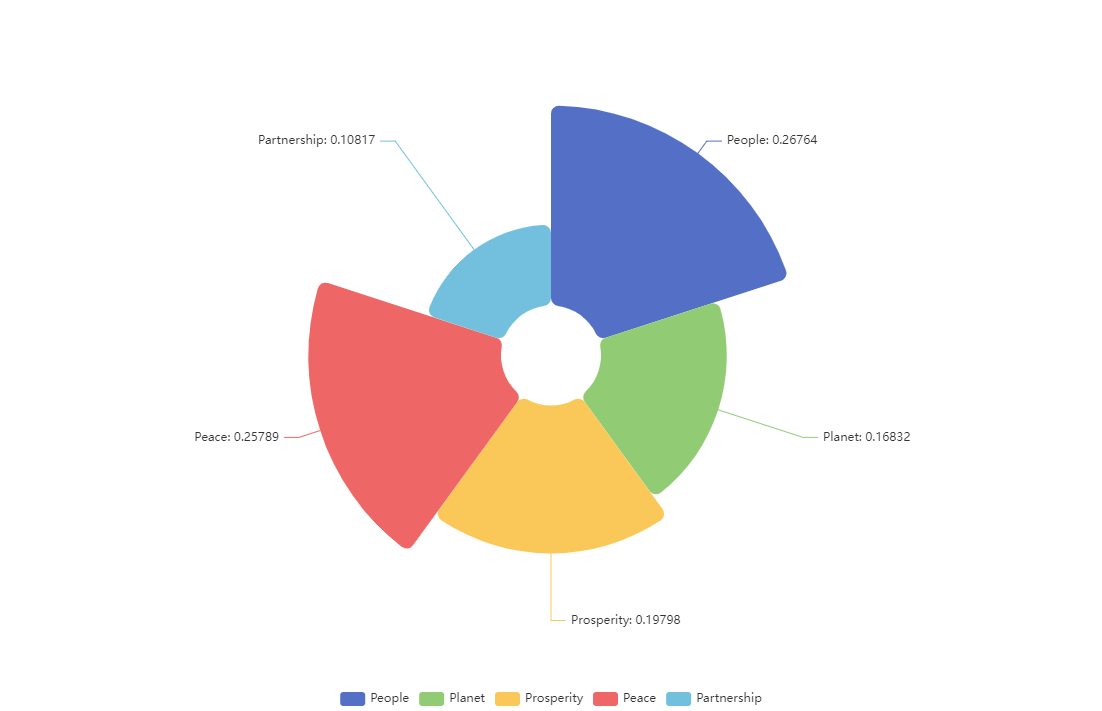
\includegraphics[scale=0.40]{{figure/PIE-Zhengzhi.png}}%插入图片的指令
    \caption{Weights under the influence of political factors}%标题
    \label{Label}
\end{figure}


Based on this matrix, we can obtain the final numerical values:
\begin{table}[h]
\centering
\begin{tabular}{|c|c|}
  \hline
  Category & Weight \\
  \hline
  People & 0.26764 \\
  Planet & 0.16832 \\
  Prosperity & 0.19798 \\
  Peace & 0.25789 \\
  Partnership & 0.10817 \\
  \hline
\end{tabular}
\caption{Weights for the 5 Ps with updated values}
\label{tab:updated_weights}
\end{table}




\subsubsection{Others}

\begin{table}[h]
\centering
\begin{tabular}{|c|c|c|c|}
\hline
Category & Environment & Technology & Economy \\
\hline
People & 0.35 & 0.2969 & 0.20 \\
Planet & 0.19 & 0.1693 & 0.13 \\
Prosperity & 0.22 & 0.2382 & 0.43 \\
Peace & 0.13 & 0.1608 & 0.09 \\
Partnership & 0.11 & 0.1348 & 0.15 \\
\hline
\end{tabular}
\caption{Combined weights for environment, technology economy}
\label{tab:combined_weights}
\end{table}
\begin{figure}[h]%插入图片并且加上图片的标题,这是一个模板
    \centering
    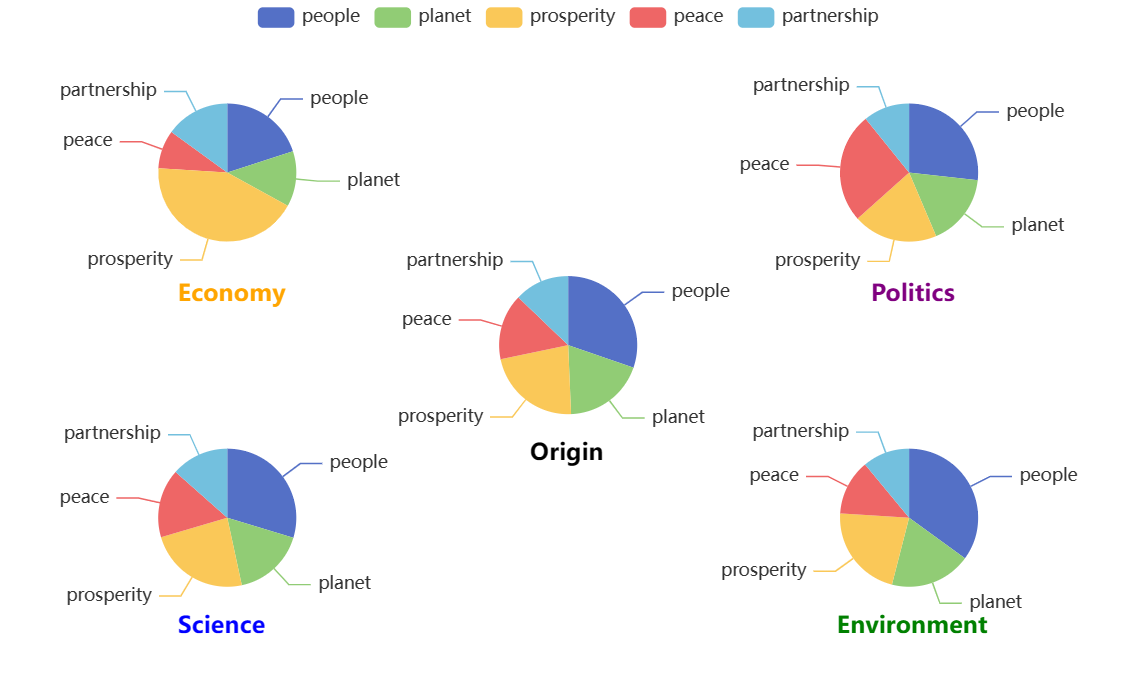
\includegraphics[scale=0.35]{{figure/Task4_Charts.png}}%插入图片的指令
    \caption{Pie Charts: Combined Weights of Origin, Economy, Science, Politics, Environment}%标题
    \label{Label}
\end{figure}



Environmental issues can lead to climate change, economic recession or depression, social unrest or conflict, and so on. Therefore, such weight ratios were derived.

When significant scientific and technological progress emerges, it can be seen that compared to the original weights, the weight of People decreases slightly, while the weight of Prosperity increases slightly, with relatively little relative change in the other three Ps.

When encountering economic depression and other issues, it will have a profound impact on global trade, industry, and employment.

%%%%%%%%%%%%%%%%%%%%%%%%%%%%%%%%%%%%%%%%%%%%%%%%%%%%%%%%%%%%%%%%%%%%%%%%%%%%%%
\section{Task5: Application of Predictive Modeling Methods in Organizational Decision Making}


%讨论你的网络方法如何帮助其他公司和组织设定目标的优先级。
% 首先,其他公司和组织可以通过类似任务一中的网络对各项目标的相互关系进行阐述;同时还可以根据对目标的初步分类,来为代表这些目标的点上色。这种网络图的模板有助于其他公司和组织去明确自己所需要完成的目标之间的关系,同时对于同类的目标也可以通过相同的颜色进行标记。
First, other companies and organizations can elaborate on the interrelationship of the goals through a network similar to the one in Task 1; they can also color the dots representing the goals based on an initial categorization of the goals. This network diagram template helps other companies and organizations to clarify the relationship between the goals they need to accomplish, and to mark similar goals with the same color.

% 其次,我们组使用的K-Means算法和AHP结合的优先事项确定机制,对于其他的组织和企业也有着可以借鉴的作用。比如当这些组织和企业的决策层涉及比较多的事项的时候,我们可以使用K-Means算法来进行决策层各个事项的分类,然后用根据分类把拆分过后的各个目标分别放进AHP的决策层中,这样子就可以减少工作量,也会使得运算出的结果更加地科学。
Second, the \textbf{K-Means algorithm} and \textbf{AHP} used by our group can be useful for other organizations and enterprises. For example, when the decision level of these organizations and enterprises involves more issues, we can use the K-Means algorithm to classify each issue in the decision level, and then use the classification to put the split objectives into the decision level of AHP, which can reduce the workload and make the results more scientific.


% 同时我们认为,这些公司和组织可能也会遇到另一种情况:就比如说这些公司的决策层中的各项指标可能所赋予的权值方差比较大,有的可能很大,有的可能远小于其他的指标。虽然我们在这些任务中并没有遇到这种情况,所有的评价指标的重要性均没有出现“远小于其他指标”的情况。但是这种情况也是值得考虑的。

% 我们觉得如果出现这种情况的话,可以通过类似“剪枝”的方法,将权重远小于其他决策层指标的那些指标统统去掉,这样子一方面由于这些指标的权重相对较小,对于最终的决策其实没有太大的影响,另一方面这样子也可以让决策层和方案层之间的矩阵数量减少,从而进一步提高了运算的速率。
At the same time, we believe that these companies and organizations may also encounter another situation: for example, the variance of the weights assigned to the indicators at the decision-making level in these companies may be large, some may be large, and some may be much smaller than others. Although we did not encounter this situation in these tasks, none of the evaluation indicators had a "much smaller importance" than the others. However, it is worth considering this situation.


\begin{figure}[h]%插入图片并且加上图片的标题,这是一个模板
    \centering
    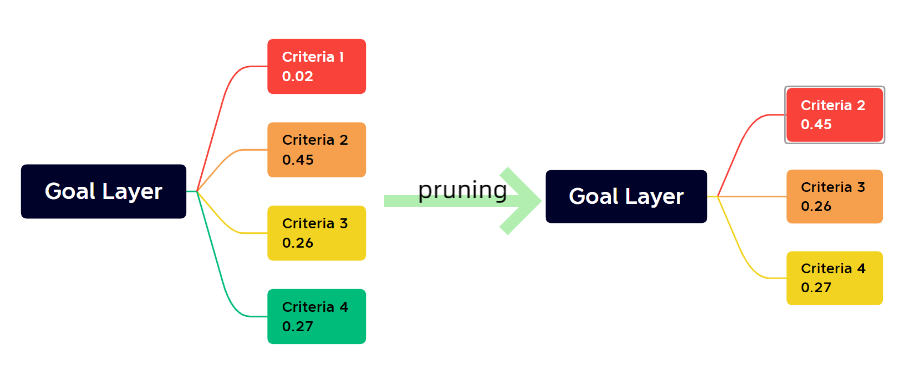
\includegraphics[scale=0.42]{{figure/Task5_Pruning.png}}%插入图片的指令
    \caption{Pruning of Unimportant Criteria Elements}%标题
    \label{Label}
\end{figure}


We think that if this situation occurs, we can remove all the indicators that have much less weight than other indicators at the decision level by a method similar to "pruning", so that on the one hand, the weight of these indicators is relatively small and has little impact on the final decision, and on the other hand, the number of matrices between the decision and solution levels can be reduced. The number of matrices between decision and solution layers is reduced, which further improves the speed of computation.


% 在这里我们认为,如果某一项指标计算出来的全职是其他指标平均值的1/10,那么我们就可以认定其为“影响微小的指标”,因而不去考虑它;在计算平均值的时候,只选择那些看上去权值比较大的那些指标,而小指标的大小均不考虑运算进去;但是如果小指标过多从而导致每个小指标相加所占的权重会占到总权重的相对比较大的份额,则可以考虑适当地通过一些合并的手段来进行这些指标的合并。
Here we think that if the full time of a certain indicator is 1/10 of the average of other indicators, then we can consider it as a \textbf{"small impact indicator"} and do not consider it; when calculating the average, only those indicators that seem to have a relatively large weight are selected, and the size of small indicators are not considered in the calculation.

\section{Extend Our Model}


%%%%%%%
%我们任务一中的模型中选取的是比较小范围的温度来进行模型的拟合,因为上海崇明岛是属于亚热带季风性气候,因此全年的温差不大,大部分时候的温度集中在10摄氏度到30摄氏度内。不过如果考虑到可能在冬季的零下低温和夏季的高温对植物中各种酶的损伤,从而导致的后续植物生长的变缓甚至停滞,本模型就没有涉及对这一方面的讨论;不过由于我们后来要研究的是在集装箱内的植物生长模型,那么这一不足就显得无关紧要了。对于光照也是同样的道理,讨论适宜范围的光照强度即可。   
%任务二中,我们考虑了单个个体吸收的土地资源,因为单个个体受到单株土地占有量(即总土地面积除以种植密度)的影响并非线性关系,因此需要先把这种影响单独拿出来进行分析。当然,对于不同的土地或者培养皿其对应的函数是不一样的,我们这里是选了一种特定的培养环境进行分析;如果有更换培养环境的需要则可以进一步分析:如不使用土地栽培而是用培养皿分瓶栽培,那么这里对于种植密度的讨论就只局限于光照竞争而不考虑营养成分竞争了,当然土地培养和培养皿培养本身的成本就有不同,这里我们还是选用成本较低的土地培养。同时在本模型中我们考虑的是使得在收获100-200g生菜的条件下的最大收获量,那么对于蔬菜的品质、口味就没有过多的考虑:当然了,如果在某一个生长阶段的生菜口味较好,容易出售的话,我们也可以据此调整收获时间。

%在任务三中,我们终于引入了温控和光控系统对于集装箱的温度的调节。此时的光强和温度都是根据模型一里的最优值进行设定的;当然,对于植物来说,适宜的温度和光强不只有一组数值,而是一个范围,因此如果对降低能源损耗有着更高的要求,那么我们可以给温度设定一个区间值,比如低温的时候让箱内温度大于等于一个最小值,高温的时候让温度小于等于一个最大值,如果外部气温处于该温度区间则可以减少甚至停止空调的使用。本次的集装箱使用的是不透光的集装箱,因而生菜所需光照均由内部灯光解决:如果考虑使用玻璃外壳集装箱,那么光照的耗能就会相应地减少,但是在高温暴晒天气下的调温功率就会显著上升。考虑到空调的耗电远高于电灯的耗电,那么我们还是尽量以增加光照能耗为代价去尽量减少空调的能耗,因而不使用透明集装箱。

%%%%%%%
%Task 1
\begin{itemize}
    \item \textbf{Model I:}
    
    The model in \textbf{Task 1} was fitted to a relatively small range of temperatures because Chongming Island, Shanghai, has a subtropical monsoonal climate, so there is little temperature difference throughout the year, with most of the time the temperature ranges from 10 to 30 degrees Celsius.

    However, if we consider the possible damage to various enzymes in the plants due to subzero temperatures in winter and high temperatures in summer, which may slow down or even stagnate the subsequent plant growth, this aspect is not discussed in this model; however, since we will later study the plant growth model in containers, this deficiency is irrelevant. The same holds for light, and it is sufficient to discuss the appropriate range of light intensities. 
    
    \item \textbf{Model II:}
    
    In \textbf{Task 2}, we considered the land resources absorbed by individual individuals, because the influence of individual individuals by the amount of land occupied by a single plant (i.e., a total land area divided by planting density) is not linearly related, so this influence needs to be taken out separately for analysis first. Of course, the corresponding function is different for different land or Petri dishes, and we have chosen a specific cultural environment for analysis here; if there is a need to change the cultural environment, then further analysis can be done: if instead of land cultivation, Petri dishes are used for vial cultivation, then the discussion of planting density here is limited to light competition without considering the nutrient competition. 

    Of course, the cost of land culture and Petri dish culture itself is different, so here we still choose the lower cost of land culture. Also in this model, we consider the maximum harvest volume under the condition of harvesting 100-200g of lettuce, so we do not consider too much about the quality and taste of the vegetables: of course, if the lettuce is at a certain growth stage tastes better and is easy to sell, we can adjust the harvest time accordingly.
    
    \item \textbf{Model III:}
    
    %Task 3
    In \textbf{Task 3}, we finally introduced the temperature control and light control system for the regulation of the container temperature. At this time, the light intensity and temperature are set according to the optimal values in Model 1; of course, for plants, the appropriate temperature and light intensity is not just a set of values, but a range, so if there are higher requirements for reducing energy losses, then we can set an interval value for the temperature, such as low temperature so that the temperature inside the box is greater than or equal to a minimum value, a high temperature so that the temperature is less than or equal to A maximum if the external temperature is in the temperature range can reduce or even stop the use of air conditioning.
    
    The container used in this case is opaque, so the light required for lettuce is solved by the internal light: if we consider using a glass shell container, the energy consumption of light will be reduced accordingly, but the power of temperature regulation will be significantly increased in hot and sunny weather. Considering that the power consumption of air conditioning is much higher than the power consumption of electric lights, then we still try to increase the energy consumption of light at the expense of minimizing the energy consumption of air conditioning, and therefore do not use transparent containers.
    
\end{itemize}
  

%Task 2


\section{Appendices}
\subsection{Appendices 1}
\lipsum[1-2]
\subsection{Appendices 2}
\lipsum[1-2]



%\section{References}
\begin{thebibliography}{99}
	\bibitem{1}Shiping Cheng, Ming Chen and Yue Ying, The combination of AHP and K-means clustering Method for determining the weight of evaluation indicators for doctoral dissertations,Changsha Hunan: Graduate School of Central South University, 2021:2-3
    \bibitem{2}SDGs.Wikipedia: https://en.wikipedia.org/wiki/
    \bibitem{3}Our World in Data: https://ourworldindata.org/
    \bibitem{4}Statista: https://www.statista.com/
	\bibitem{5}The UN:https://sdgs.un.org/goals
	\bibitem{6}Bojie Fu, Shuai Wang, Junze Zhang, Zengqian Hou, Jinghai Li, Unravelling the complexity in achieving the 17 sustainable-development goals, National Science Review, Volume 6, Issue 3, May 2019, Pages 386–388, https://doi.org/10.1093/nsr/nwz038
	\bibitem{7}George Halkos, Eleni-Christina Gkampoura,
    Where do we stand on the 17 Sustainable Development Goals? An overview on progress,
    Economic Analysis and Policy,
    Volume 70,
    2021,
    Pages 94-122,
    ISSN 0313-5926,
    https://doi.org/10.1016/j.eap.2021.02.001.
    \bibitem{8}Luis Ospina-Forero, Gonzalo Castañeda, Omar A. Guerrero,
    Estimating networks of sustainable development goals,
    Information and Management,
    Volume 59, Issue 5,
    2022,
    103342,
    ISSN 0378-7206,
    https://doi.org/10.1016/j.im.2020.103342.
    \bibitem{9}Bellantuono, L., Monaco, A., Amoroso, N. et al. Sustainable development goals: conceptualization, communication and achievement synergies in a complex network framework. Appl Netw Sci 7, 14 (2022). https://doi.org/10.1007/s41109-022-00455-1
    \bibitem{10}Our \textbf{ANONYMOUS} Code Repository:https://anonymous.4open.science/r/MCM-2023-2321591-Codess-740F

\end{thebibliography}





%%%%%%%%%%%%%%%%%%%%%%%%%%%%%%
\end{document}
\end